\section{Implementation and Experimental Setup}
\label{subsec:eval-setup}

% \junchen{need to update}

\mypara{Implementation}
\name uses PyTorch~\cite{pytorch} for running and training ML models, and each component is implemented as a collection of long-running processes with the Ray\cite{ray} actor model. The micro-profiler and training/inference jobs run as independent actors which are controlled by the thief scheduler actor. \name achieves fine-grained and dynamic reallocation of GPU between training and inference processes using Nvidia MPS~\cite{nvidia-mps}, which provides resource isolation within a GPU by intercepting CUDA calls and rescheduling them. Our implementation also adapts to errors in profiling by reactively adjusting its allocations if the actual model performance diverges from the predictions of the micro-profiler. \name's code and datasets are available at the project page: \href{https://aka.ms/ekya}{aka.ms/ekya}

\mypara{Datasets} 
We use both on-road videos captured by dashboard cameras as well as urban videos captured by mounted cameras. The dashboard camera videos are from cars driving through cities in the US and Europe, Waymo Open~\cite{waymo} (1000 video segments with in total 200K frames) and Cityscapes~\cite{cityscapes} (5K frames captured by 27 cameras) videos. The urban videos are from stationary cameras mounted in a building (``Urban Building'') as well as from five traffic intersections (``Urban Traffic''), both collected over 24-hour durations. % and a set of 24-hour urban traffic videos (``Urban Traffic'') captured by 5 cameras. %\junchen{add bellevue dataset once it's included}
% For our evaluation, we use the Waymo Open\cite{waymo} and Cityscapes\cite{cityscapes} datasets, two popular video datasets containing dashboard camera footage of cars driving through cities in the US and Europe. Cityscapes has frames from 27 video streams training with a total of 5000 pixel-level annotated frames, while Waymo Open has 1000 video segments with a total of 200000 frames.
We use a retraining window of 200 seconds in our experiments, and split each of the videos into 200 second segments.  
%The traffic videos are captured continuously and we split them into 200-second retraining windows. 
Since the Waymo and Cityscapes dataset do not contain continuous timestamps, we 
%However, the two public datasets %organize their images chronologically but 
%do not contain continuous timestamps.We 
create retraining windows by concatenating images from the same camera in chronological order to form a long video stream and split it into 200 second segments. %10 retraining windows. 
% in Cityscapes, treating a block of consecutive \fillme images from the same video source (in total 27 sources); and (2) in Waymo, concatenating 20s-video segments belonging to the same source in chronological order.
% The workload in Cityscapes is constructed by treating each city's video as an independent video stream feeding into {\name} for inference and retraining. The workload in Waymo Open is constructed by creating video streams by concatenating 20s-video segments belonging to the same city in chronological order. Each video stream in both datasets is then split into 10 retraining windows. 
%%GA While these images may not be captured at a uniform interval over time, they show representative workloads of independent video streams with local variations which necessitate retraining for their specific data-distributions.


% \mypara{DNN models}
% \revtext{
% We evaluate \name{} on two separate machine learning tasks - object classification and object detection. Our experiments run on a diverse set of edge DNNs - ResNet18\cite{deepresidual-2}, MobileNetV2\cite{compression-17} and SqueezeNet\cite{compression-18} for object classification and TinyYOLOv3\cite{redmon2018yolov3} and SSD\cite{liu2016ssd} for object detection. As explained in \S\ref{subsec:continuous}, we use an expensive golden model (ResNeXt 101 \cite{wang2019elastic} for object classification and YOLOv3 \cite{redmon2018yolov3} for object detection.) to get ground truth labels for training and testing.
% %The golden model-produced labels are also used as ground truth to evaluate inference accuracy.
% On a subset of data that have human annotations, we confirm that the labels produced by the golden model are very similar to human-annotated labels.} %\romil{Golden model acc Cityscapes: 82\% Waymo: 76\%}
% % \junchen{add golden model labeling and that golden model cannot run on every image}

\revtext{
\mypara{DNNs}
We demonstrate \name's effectiveness on two machine learning tasks -- object classification and object detection -- using multiple compressed edge DNNs for each task:
$(i)$ object classification using ResNet18\cite{deepresidual-2}, MobileNetV2\cite{compression-17} and ShuffleNet\cite{shufflenet}, and $(ii)$ object detection using TinyYOLOv3\cite{redmon2018yolov3} and SSD\cite{liu2016ssd}. As explained in \S\ref{subsec:continuous}, we use an expensive golden model (ResNeXt 101 \cite{wang2019elastic} for object classification and YOLOv3 \cite{redmon2018yolov3} for object detection) to get ground truth labels for training and testing.}


% \noindent\textbf{System Implementation.}\junchen{shrink or remove given the impl section}
% We implement a prototype of \name in Python using Ray\cite{ray} for asynchronous operations and RPCs. 
% Each video stream is modelled as an independent Ray actor whose resource allocation for inference and training is periodically updated by the Ekya master.

% % Write about microprofiling
% %\mypara{Microprofiling}
% The Ekya implementation ingests video streams and splits it into evenly sized retraining periods. At the start of each retraining period, the hyperparameters are micro-profiled \ref{sec:microprofiling} and the thief scheduler is run to compute the resource allocations for training and inference jobs. 
% %This resource allocation is then enforced by Ekya by launching new training processes and restarting the inference processes with updated resource weights. 

% Ekya requires fine-grained GPU allocation between inference and training processes. 
% Talk about memory isolation in Ekya.
% Talk about nvidia MPS resource sharing

% \junchen{update once Romil finishes the impl tests}

\mypara{Testbed and trace-driven simulator}
% \junchen{update this?}
We run \name's implementation on AWS EC2 p3.2xlarge instances for 1 GPU experiments and p3.8xlarge for 2 GPU experiments. Each instance has Nvidia V100 GPUs with NVLink interconnects. %and Intel Skylake Xeon processors.   % Nvidia RTX 2080 and Intel Xeon E-2226G CPU.

%To complement the system implementation, 
% In addition to the system implementation \cref{sec:system}, 
We also built a simulator to %scale out the test of training and inference jobs to 
test \name under a wide range of resource constraints, workloads, and longer durations. 
The simulator takes as input the accuracy and resource usage (in GPU time) of training/inference configurations logged from our testbed. 
% The inputs to the simulator are execution traces from training and inference workloads with different configurations.
%To collect execution traces, we ran all configurations on the 10 retraining windows for every video stream in the three datasets. 
For each training job, we log the accuracy over GPU-time. We also log the inference accuracy on the real videos. %\gaa{Once the model is trained, we also log its test accuracy over the future retraining windows to get the accuracy in future windows if it was not retrained.} 
This exhaustive trace allows us to mimic the jobs with high fidelity under different scheduling policies. %simulate custom scheduling policies, modify the execution order, simulate resource sharing and allocation. 

% Talk about the assumptions - inference accuracy min GPU, linear scaling etc

\mypara{Retraining configurations}
% \junchen{shrink it. just need to list the hyperparameters. one question though: inference configs?}
%For each training job, we create a fixed set of configurations by varying the values of following hyperparameters - number of epochs to train, batch size, number of neurons in the last layer, number of layers to retrain, and the fraction of data between retraining windows to be used for retraining. We then selected combinations of these hyperparameters to create a diversity in the resource-accuracy profiles of the configurations. 
Our retraining configurations combine the number of epochs to train, batch size, number of neurons in the last layer, number of layers to retrain, and the fraction of data between retraining windows to use for retraining (\S\ref{subsec:profiles}). 
% \revtext{To constrain the memory utilization of the object detection models (TinyYOLO and SSD), we limit the batch size to 8 and aggressively set the fraction of layers to retrain between 0.1 and 0.3.}
\revtext{For the object detection models (TinyYOLO and SSDLite), we set the batch size to 8 and the fraction of layers frozen between 0.7 and 0.9. The resource requirements of the configurations for the detection models vary by $153\times$.} 
% \ga{(1) Do we have to ``fit'' because of memory constraint?; (2) Would it be a good idea to include resource-accuracy profiles for detectors? \S\ref{subsec:profiles} does not talk about detectors.}

% \junchen{mention the edge DNNs}

% \mypara{Performance metrics}
% \junchen{tbd: accuracy, throughput (\# of streams) under given \# of gpus}


\mypara{Baselines}
%To focus our evaluation on \name's scheduling strategy, we 
Our baseline, called {\em \fair scheduler},  %retrains the models in the same way as \name except it
uses $(a)$ a fixed retraining configuration, and $(b)$ a static retraining/inference resource allocation (these are adopted by prior schedulers \cite{fair-1, fair-2, videostorm}). 
For each dataset, we test all retraining configurations on a hold-out dataset \footnote{
The same hold-out dataset is used to customize the off-the-shelf DNN inference model. This is a common strategy in prior work (\eg~\cite{noscope}).} (\ie two video streams that were never used in later tests) to produce the Pareto frontier of the accuracy-resource tradeoffs %over all retraining configurations 
(\eg Figure~\ref{fig:resource-profiles}). 
The \fair scheduler then picks two points on the Pareto frontier as the fixed retraining configurations to represent ``high'' (Config 1)  and ``low'' (Config 2) resource usage, and uses one of them for all retraining windows in a test.
%The \fair scheduler then picks three points on the Pareto frontier as the fixed retraining configurations to represent ``high'', ``medium'', and ``low'' resource usage, and uses one of them for all retraining windows in a test.
%The gains of \name compared to this \fair scheduler reflects the benefit of the {\name}'s %thief scheduler and the microprofiler that 
%intelligent allocation of resources among models of video streams and adapting the schedule over time to maximize overall inference accuracy.

We also consider two alternatives in \S\ref{subsec:eval-alternate}. 
(1) {\em offloading retraining to the cloud}, and %so that the edge servers can focus on inference, and 
(2) {\em caching and re-using a retrained model} from history based on various similarity metrics.
% \revtext{based on similarity in the time-of-day, location, distribution of classes, and number of objects.}
% \revtext{which swaps models based on different criteria, such as time-of-day, location, class-distribution similarity and number of objects in the scene.} %that shares class distribution (instead of retraining the model again).
%We will present their details in \S\ref{subsec:eval-alternate}.


% against a weighted {Fair Scheduler} \cite{fair-1, fair-2, videostorm}, which allocates equal resources to all video streams and within a video stream, allocates resources to training and inference proportional to the weight set as the \lstinline{inference_weight} parameter to scheduler. A higher \lstinline{inference_weight} implies a higher resource allocation to inference and a reduced allocation to training jobs. To pick retraining hyperparameters, the fair scheduler employs the common heuristic of highest-accuracy first. 

%We compare against two baselines. First is \textit{No-retraining}, which does not ever retrain the model and thus allocates resources only to inference. Second is \textit{Fair Scheduler} \cite{fair-1, fair-2, videostorm} which allocates equal resources to all video streams and within a video stream, allocates equal resources to both, training and inference. To pick retraining hyperparameters, the fair scheduler employs the common heuristic of highest-accuracy first. 
% Why are these good baselines?

% \textbf{Metrics.}
% % More:
% Our most used metric is Inference Accuracy over time, as described in \S\ref{subsec:formulation}. We also use the number of GPUs provisioned at the edge server as a measure of cost.



% 6.2 Overall improvement

% - accuracy vs. gpus (fix \# of videos)

% - streams vs. gpus (fix accuracy)

% - accuracy vs. streams (fix \# of gpus)

% - alternative architectures


\section{Evaluation}
\label{sec:evaluation}

%\subsection{Evaluation Highlights}
We evaluate \name's performance, and the key findings are:
% on the Waymo and Cityscapes data. %The highlights are:

%\begin{packeditemize}
%\item 
\noindent{\bf 1)} Compared to static retraining baselines, \name achieves upto 29\% higher accuracy 
\revtext{for compressed vision models in both classification and detection}. 
% \revtext{across a diversity of models in object detection and object classification}. 
For the baseline to match \name's accuracy, it would need $4\times$ additional GPU resources. (\S\ref{subsec:eval:overall}) %(for same set of video streams) 
% or process 2$\times$ video streams (under the same inference accuracy target) 
%when given the same amount of provisioned resource. To achieve the same accuracy as \name, the baselines require 4$\times$ more GPU resources.
%\item 

\noindent{\bf 2)} Both micro-profiling and thief scheduler contribute sizably to \name's gains. (\S\ref{subsec:eval-understanding}) 
In particular, the micro-profiler estimates accuracy with low median errors of $5.8\%$. %to allow the thief scheduler pick the best-performing configurations.
(\S\ref{subsec:eval-profiling})
%\item 

\noindent{\bf 3)} The thief scheduler efficiently makes its decisions in 9.4s when deciding for 10 video streams across 8 GPUs with 18 configurations per model for a 200s retraining window. (\S\ref{subsec:eval-understanding})

\noindent{\bf 4)} Compared to alternate designs, 
% including retraining the models in the cloud or \revtext{swapping pre-trained models based on scenarios}, 
including \revtext{reusing cached history models trained on similar data/scenarios} as well as retraining the models in the cloud,
\name achieves significantly higher accuracy without the network costs (\S\ref{subsec:eval-alternate}).
    % \item With multiple cameras sharing the resources on an edge server, \name{} achieves upto \romilc{16}\% \romil{This is sim, check exact with zhengxu} points higher accuracy than the fair sharing baseline. Attaining the same accuracy with a fair-sharing scheduler would require upto \romilc{$2.xx\times$} more resources.
    % \item With the same resource provisioning, \name{} is able to support upto $5\times$ more video streams than the fair scheduler.
    % \item \name{}'s performance gracefully degrades with reduction in resources to the baseline that does not retrain since it evaluates the cost of retraining on the accuracy. 
%\end{packeditemize}

\subsection{Overall improvements}
\label{subsec:eval:overall}


We evaluate \name and the baselines along three dimensions---
\revtext{
{\em inference accuracy} (\% of images correctly classified for object classification, F1 score (measured at a 0.3 threshold for the Intersection-over-Union of the bounding box) for detection),}
{\em resource consumption} (in GPU time), and {\em capacity} (the number of concurrently processed video streams).
Note that the evaluation always keeps up with the video frame rate (\ie no indefinite frame queueing). 
{\revtext{By default we evaluate the performance of Ekya on ResNet18 models, but we also show that it generalizes to other model types and vision tasks.}}
% \revtext{We evaluate the performance of Ekya with the ResNet family of models and generalize our results across other model types.}
% \junchen{did you mean still keeping up with 30 fps?}\romilc{Yes.}
%Here, we show that \name achieves better tradeoffs between two of these metrics while the third dimension is fixed.



% Sys Impl result
\begin{figure}[t]
\captionsetup[subfigure]{justification=centering}
  \centering
  \begin{subfigure}[t]{0.9\linewidth}
    \centering
    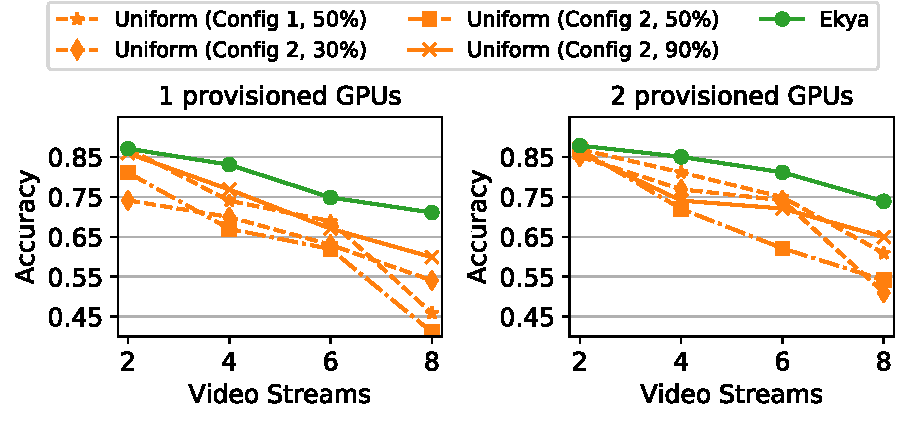
\includegraphics[width=\linewidth]{ekya/results/sys_impl/sysimpl_varyingcities_streams_cityscapes.pdf}
    \caption{\small Cityscapes}
    \label{fig:sys-impl-cityscapes}
  \end{subfigure}
  \\
  \begin{subfigure}[t]{0.9\linewidth}
    \centering
    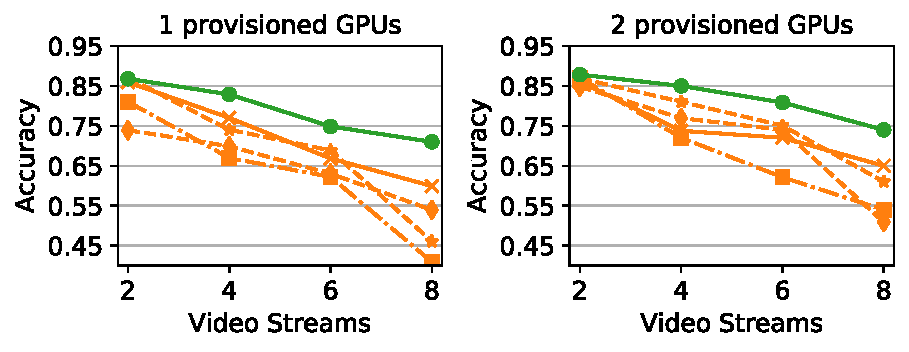
\includegraphics[width=\linewidth]{ekya/results/sys_impl/sysimpl_varyingcities_streams_waymo.pdf}
    \caption{\small Waymo}
    \label{fig:sys-impl-waymo}
  \end{subfigure}
  ~~~
%   ~
%   \begin{subfigure}[t]{0.45\linewidth}
%     \centering
%     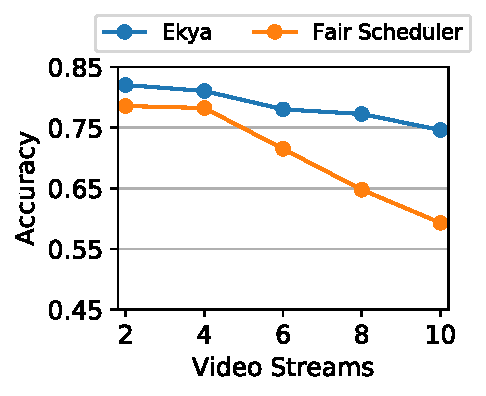
\includegraphics[width=\linewidth]{results/sys_impl/sysimpl_varyingcities_streams_cityscapes_2gpu.pdf}
%     \caption{\small Two provisioned GPUs}
%     \label{fig:sys-impl-2gpu}
%   \end{subfigure}
%   ~
%   \begin{subfigure}[t]{0.3\linewidth}
%     \centering
%     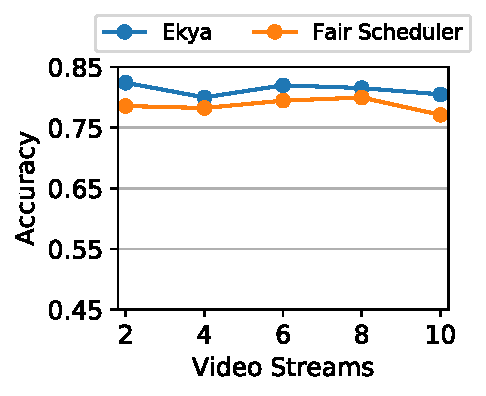
\includegraphics[width=\linewidth]{results/sys_impl/sysimpl_varyingcities_streams_cityscapes_4gpu.pdf}
%     \caption{\small 4 GPU}
%     \label{fig:sys-impl-4gpu}
%   \end{subfigure}
  \caption{\small \bf  Effect of adding video streams on accuracy with different schedulers. When more video streams share resources, \name's accuracy gracefully degrades while the baselines' accuracy drops faster. (``Uniform (Cfg 1, 90\%)'' means the \fair scheduler allocates 90\% GPU to inference, 10\% to retraining)
    % Effect of adding more video streams on accuracy for different schedulers. When insufficient resources are provisioned, \name{} gracefully degrades to the No-retrain baseline, while the retraining decisions made by the fair scheduler reduce the mean inference accuracy.
  }
  \label{fig:scalability-sysimpl-fixedGPUs-accuracy}
\end{figure}

\mypara{Accuracy vs. Number of concurrent video streams}
Figure~\ref{fig:scalability-sysimpl-fixedGPUs-accuracy} shows the \revtext{ResNet18 model's} accuracy with \name and the baselines when analyzing a growing number of concurrent video streams under a fixed number of provisioned GPUs for Waymo and Cityscapes datasets. 
The \fair baselines use different combinations of pre-determined retraining configurations and resource partitionings. \cameratext{For consistency, the video streams are shuffled and assigned an id (0-10), and are then introduced in the same increasing order of id in all experiments. This ensures that different schedulers tested for $k$ parallel streams use the same $k$ streams, and these $k$ streams are always a part of any $k'$ streams ($k' > k$) used for testing.}
%%GA We create multiple video streams by replicating one video stream from Cityscapes dataset, in order to avoid inter-stream variations as more video streams are added.
% To minimize the accuracy variations between cities, we add video streams by replicating a fixed video stream from the Cityscapes dataset.

As the number of video streams increases, \name enjoys a growing advantage (upto 29\% under 1 GPU and 23\% under 2 GPU) in accuracy over the \fair baselines. 
This is because \name gradually shifts more resource from retraining to inference and uses cheaper retraining configurations. %, in favour of keeping a high inference accuracy while still benefiting from continuous retraining.
In contrast, increasing the number of streams forces the \fair baseline to allocate less GPU cycles to each inference job, while retraining jobs, which use fixed configurations, slow down and take the bulk of each window.
% This trend persists with different GPUs.
% With only a single provisioned GPU, 
% by allocating all resources to inference. 
% The \fair scheduler, however, is unaware of relative resource cost and benefits between the retraining and inference jobs, and thus is unable to adapt the resource allocation under different resource constraints.
% , and diverts GPU cycles from inference, resulting a lower inference accuracy.
% SIGCOMM Results:
% \begin{figure}
%  	%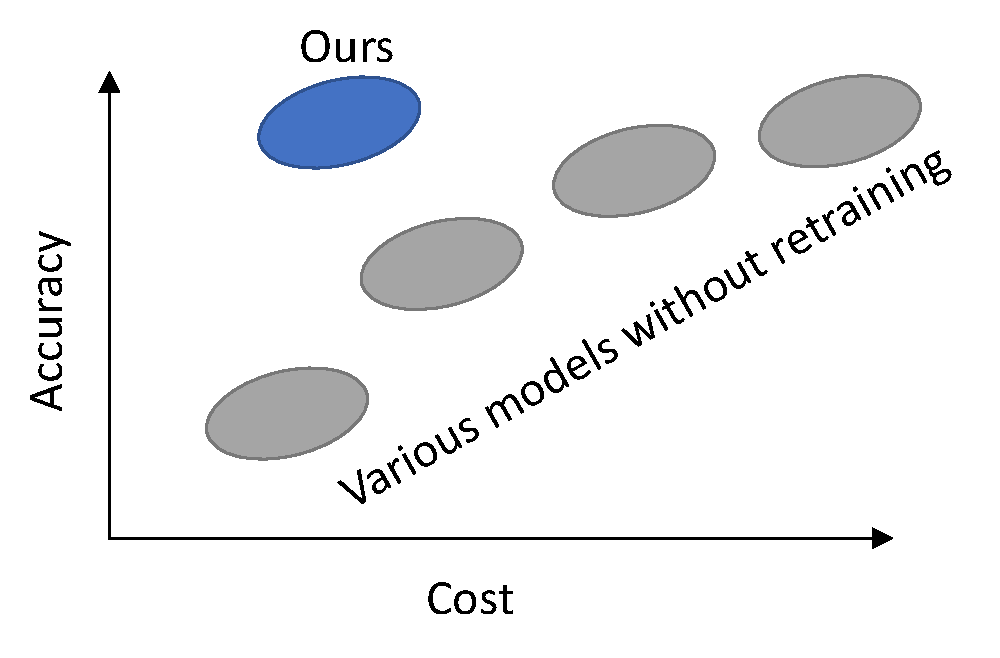
\includegraphics[width=0.4\textwidth]{ekya/figures/eval_placeholders/single-tradeoffs.pdf}
%  	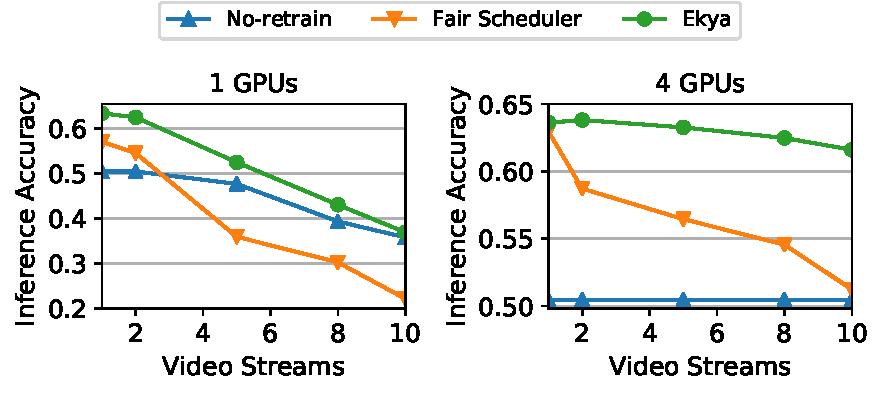
\includegraphics[width=\linewidth]{results/scalability/scalability_cams_fixedGPUs_cityscapes.pdf}
% 	\caption{\small \bf Effect of adding more video streams on accuracy for different schedulers. When insufficient resources are provisioned, \name{} gracefully degrades to the No-retrain baseline, while the retraining decisions made by the fair scheduler reduce the mean inference accuracy.}
% 	\label{fig:scalability-fixedGPUs-accuracy}
% \end{figure}
% \begin{figure}
%  	%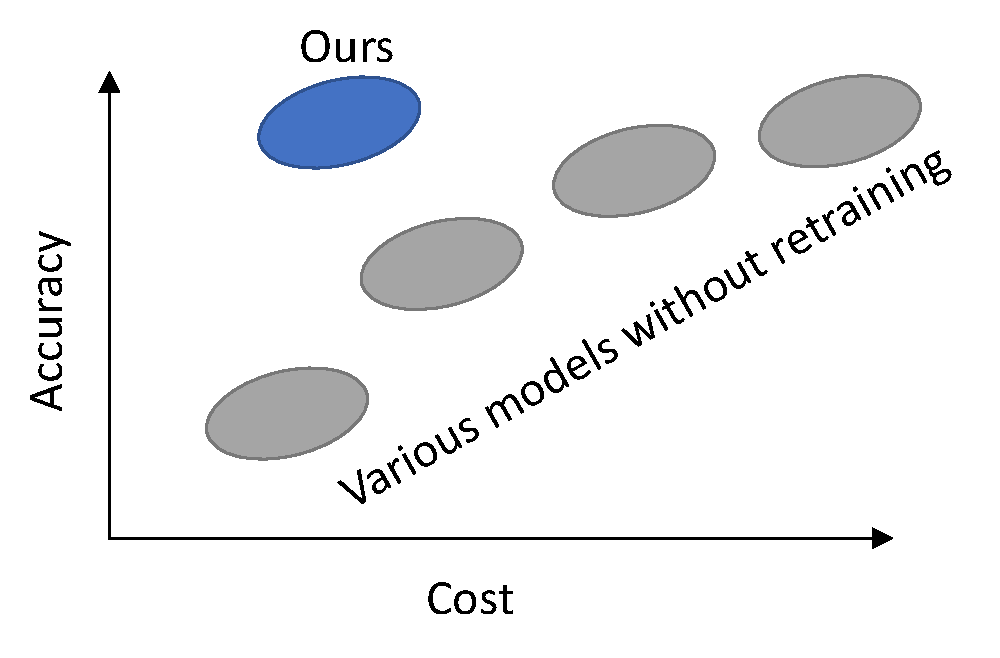
\includegraphics[width=0.4\textwidth]{ekya/figures/eval_placeholders/single-tradeoffs.pdf}
%  	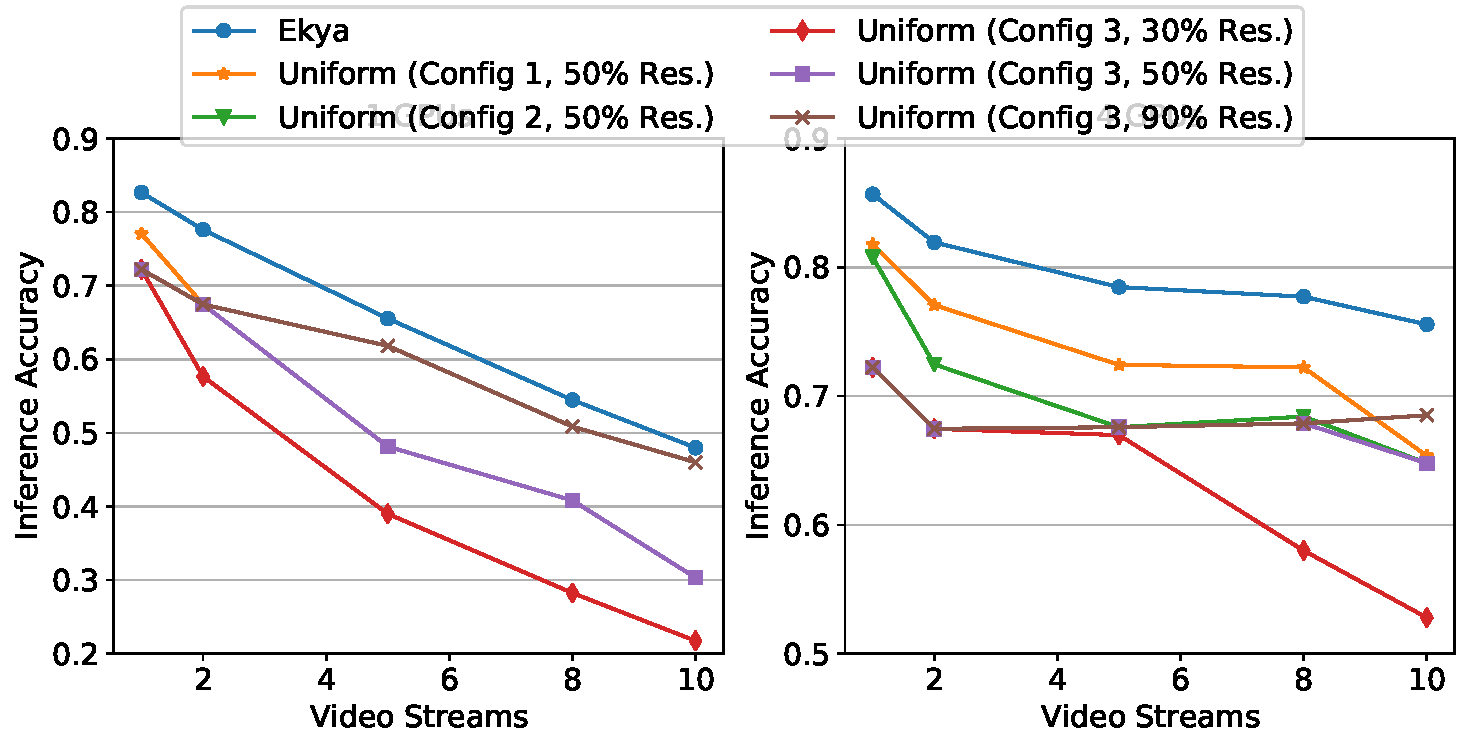
\includegraphics[width=\linewidth]{results/scalability/scalability_cams_fixedGPUs_cityscapes_golden_model.pdf}
% 	\caption{\small \bf Using Simulator. Effect of adding more video streams on accuracy for different schedulers. When insufficient resources are provisioned, \name{} gracefully degrades to the No-retrain baseline, while the retraining decisions made by the fair scheduler reduce the mean inference accuracy. \junchen{drop the ``no-retrain'' line}}
% 	\label{fig:scalability-fixedGPUs-accuracy}
% \end{figure}


\begin{table}
\footnotesize
\begin{tabular}{cccc}
\hline
\multirow{2}{*}{Scheduler} & \multicolumn{2}{c}{Capacity} & \multirow{2}{*}{Scaling factor} \\ \cline{2-3}
& 1 GPU & 2 GPUs &  \\ \hline
\textbf{Ekya} & \textbf{2} & \textbf{8} & \textbf{4x} \\ \hline
Uniform (Config 1, 50\%) & 2 & 2 & 1x \\ \hline
Uniform (Config 2, 90\%) & 2 & 4 & 2x \\ \hline
Uniform (Config 2, 50\%) & 2 & 4 & 2x \\ \hline
Uniform (Config 2, 30\%) & 0 & 2 & - \\ \hline
\end{tabular}
\caption{\small \bf Capacity (number of video streams that can be concurrently supported subject to accuracy target 0.75) vs. number of provisioned GPUs.
\name scales better than the \fair baselines with more available compute resource.
%The accuracy threshold is a multiplicative factor of the maximum achievable mean accuracy for a workload given $\infty$ resources.
}
\label{tab:scalability-gpu-vs-cam-thresholded}
%\vspace{-1em}
\end{table}

% \begin{figure}
%  	%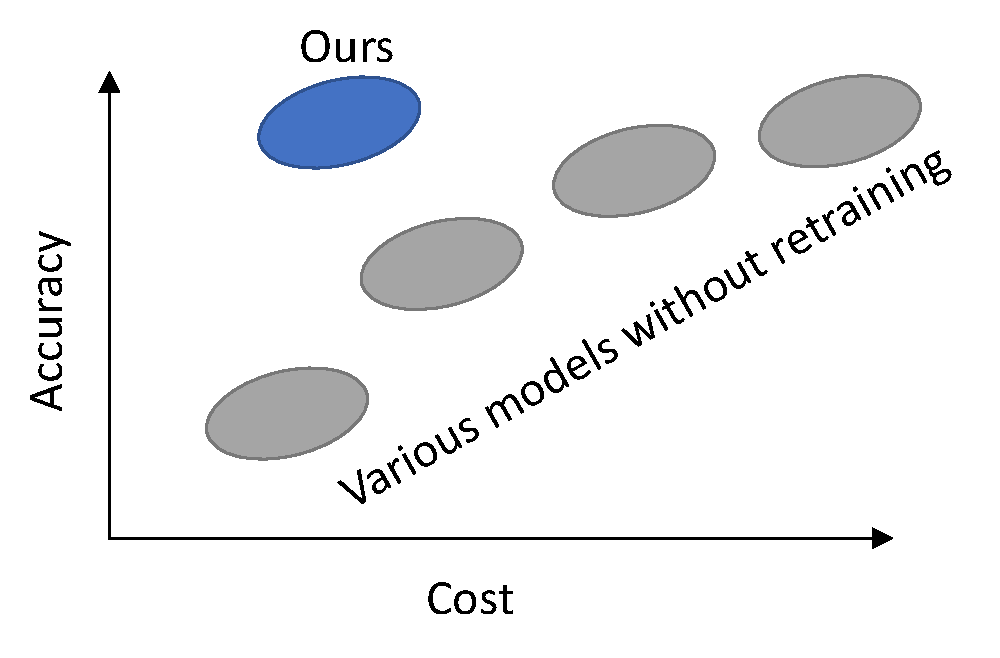
\includegraphics[width=0.4\textwidth]{ekya/figures/eval_placeholders/single-tradeoffs.pdf}
%  	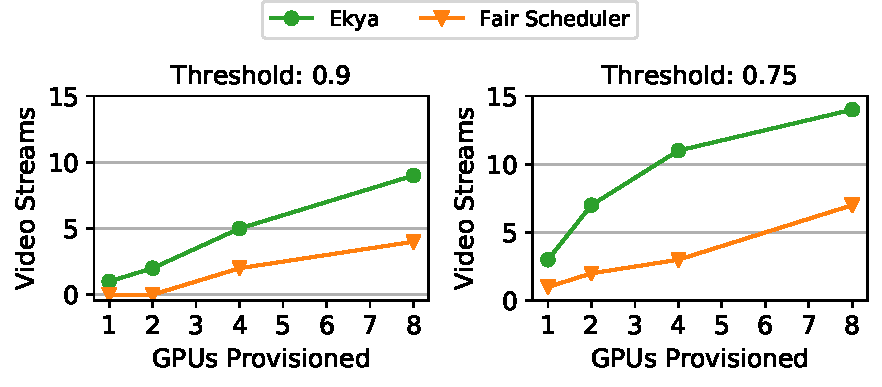
\includegraphics[width=\linewidth]{results/scalability/scalability_GPUs_cams_cityscapes.pdf}
% 	\caption{\small \bf Capacity measured as number of video streams that can be concurrently supported for different resource sizes subject to accuracy thresholds. \romil{We have just two data points per plot here with our sys impl..}
% 	%The accuracy threshold is a multiplicative factor of the maximum achievable mean accuracy for a workload given $\infty$ resources.
% 	}
% 	\label{fig:scalability-gpu-vs-cam-thresholded}
% \end{figure}



%\name's gains over no-retrain baseline are more sizable in Waymo than Cityscapes, but its gains over the fair scheduler baseline are comparable in both traces. 
%This suggests that Waymo data is inherently more suitable for continuous retraining, but through more intelligent resource allocation, \name can always squeeze more juice from retraining than fair scheduler.

% Generality result
\begin{figure}[t]
\captionsetup[subfigure]{justification=centering}
  \centering
  \begin{subfigure}[t]{0.9\linewidth}
    \centering
    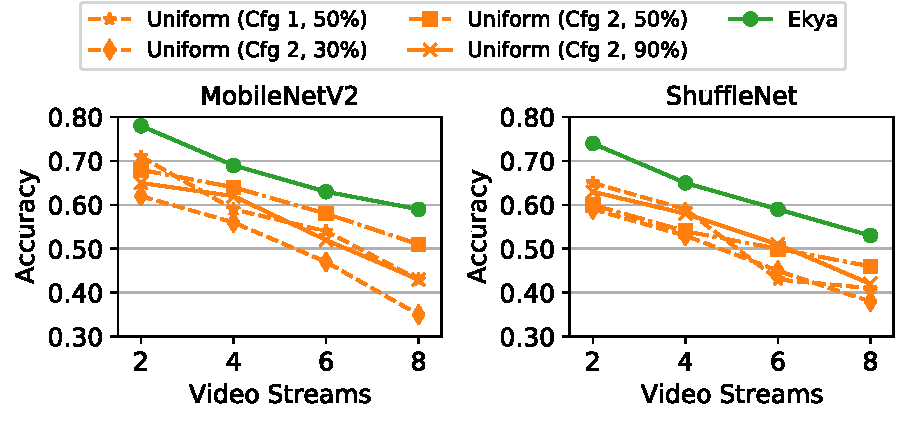
\includegraphics[width=\linewidth]{ekya/results/generality/e2e_1gpu_cityscapes_objclass.pdf}
    \caption{\small \revtext{Generalize across object classification models}}
    \label{fig:sys-impl-generality-objclass}
  \end{subfigure}
  \\
  \begin{subfigure}[t]{0.9\linewidth}
    \centering
    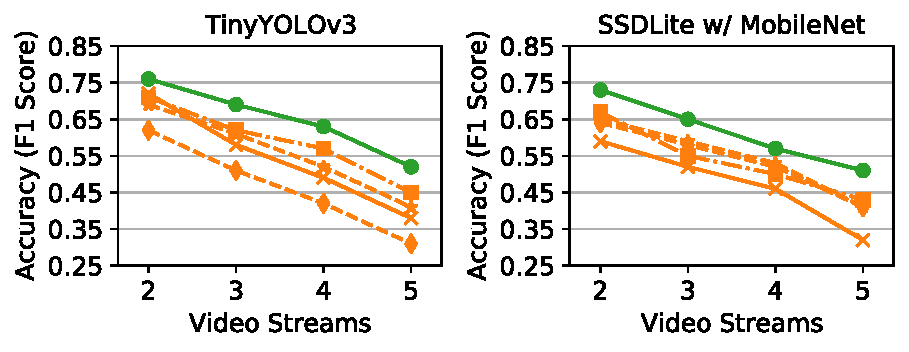
\includegraphics[width=\linewidth]{ekya/results/generality/e2e_1gpu_cityscapes_objdet.pdf}
    \caption{\small \revtext{Object Detection Models}}
    \label{fig:sys-impl-generality-objdet}
  \end{subfigure}
  ~~~
  \caption{\small \bf  \revtext{Improvement of \name extends to two more compressed DNN classifiers and two popular object detectors.
%   General applicability of \name across different ML models with varying number of video streams. 
%   \name can improve the performance of other compressed models in object classification and also extend to models in object detection.
  }}
  \label{fig:generality-models}
\end{figure}

\revtext{
\mypara{Generalizing to other ML models}
\name's thief scheduler can be readily applied to any ML model and task (e.g., classification or detection) that needs to be fine-tuned continuously on newer data. To demonstrate this, we evaluate \name with:
%many other popular object classifiers and object detectors. 

\begin{itemize}
\item {\em Other object classifiers:} Figure \ref{fig:sys-impl-generality-objclass} shows the performance of \name when running MobileNetV2 and ShuffleNet as the edge models in two independent setups for object classification at the edge. Continuing the trend that we observed for ResNet18 (in Figure~\ref{fig:scalability-sysimpl-fixedGPUs-accuracy}), Figure \ref{fig:sys-impl-generality-objclass} shows that \name leads to up to 22\% better accuracy than \fair baselines. 

\item {\em Object detection models:} In addition to object classification, we also evaluate using object detection tasks which detect the bounding boxes of objects in the video stream. 
% However, the model hyperparameter space must be carefully configured so as to ensure they still fit on the edge hardware and retrain in time. For our experiments, we reduce the batch sizes and increase the layers frozen to accommodate TinyYOLO and SSD object detection models on the edge devices.
%\junchen{i remove the sentence on limiting batch size, its repetitive to 6.1.}
Figure~\ref{fig:sys-impl-generality-objdet} shows \name outperforms the \fair baseline's F1 score by 19\% when processing same number of concurrent video streams. Importantly, \name's design broadly applies to new tasks without any systemic changes. 
\end{itemize}

These gains stem from \name's ability to navigate the rich resource-accuracy space of models by carefully selecting training and inference hyperparameters (e.g., the width multiplier in MobileNetV2, convolution sparsity in ShuffleNet). 
}
\revtext{For the rest of our evaluation, we only present results with ResNet18 though the observations hold for other models.}
% \revtext{
% \mypara{Generalizing to other ML models}
% Since the thief scheduler treats the ML model as a black box, \name can be applied on any ML task without any changes to the thief scheduler. We now demonstrate the performance of \name on a variety of models in both object detection and object classification. 

% \noindent\textbf{Model generality within object classification.} Figure \ref{fig:sys-impl-generality-objclass} shows the performance of \name when running MobileNetV2 and SqueezeNet as the edge models in two independent setups for object classification at the edge. Continuing the trend from Figure~\ref{fig:scalability-sysimpl-fixedGPUs-accuracy}, \name performs up to 22\% better than \fair baselines. Since these models are particularly designed for resource-constrained environments, they provide specific hyperparameters to trade-off accuracy for computational cost (e.g. the width multiplier parameter in MobileNetV2). This provides a rich performance-cost space for Ekya to pick configurations from, allowing it to outperform fixed configuration baselines.

% \noindent\textbf{Extending generality to object detection.} In addition to object classification, we run object detection workloads which detect the bounding boxes of objects in the video stream. Extending \name to tasks beyond object detection does not need any systemic changes to \name. However, the model hyperparameter space must be carefully configured so as to ensure they still fit on the edge hardware and retrain in time. For our experiments, we reduce the batch sizes and increase the layers frozen to accommodate TinyYOLO and SSD object detection models on the edge devices. As seen in  Figure~\ref{fig:sys-impl-generality-objdet}, \name outperforms the \fair baseline mean average precision (mAP) by 19\%.
% }


\mypara{Number of video streams vs. provisioned resource}
% scalability: with more gpus, we can support more camera
% \mypara{Scalability with more GPUs}
We compare \name's {\em capacity} (defined by the maximum number of concurrent video streams subject to an accuracy threshold) with that of \fair baseline, as more GPUs are available.
% We define throughput as the maximum number of video streams that can run concurrently on the GPUs while achieving a accuracy within a threshold of the maximum possible mean accuracy.
Setting an accuracy threshold is common in practice, since applications usually require accuracy to be above a threshold for the inference to be usable.
Table~\ref{tab:scalability-gpu-vs-cam-thresholded} uses the Cityscapes results (Figure~\ref{fig:scalability-sysimpl-fixedGPUs-accuracy}) to derive the scaling factor of capacity vs. the number of provisioned GPUs and shows that with more provisioned GPUs, \name scales faster than \fair baselines.
% : its capacity grows nearly linearly with more available GPUs, and at a rate \romilc{$2.3\times$} faster than the \fair baselines.
% This suggests that \name .






\begin{figure}
  \centering
%   \begin{subfigure}[t]{0.5\linewidth}
%     \centering
%     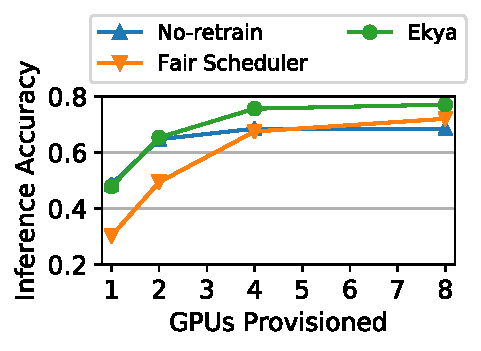
\includegraphics[width=\linewidth]{results/multicam/multicam_acc_vs_res_cityscapes.pdf} 
%     \caption{\small Cityscapes}
%     \label{fig:scalability-gpus-cityscapes}
%   \end{subfigure}
%   ~~~
%   \begin{subfigure}[t]{0.5\linewidth}
%     \centering
%     % 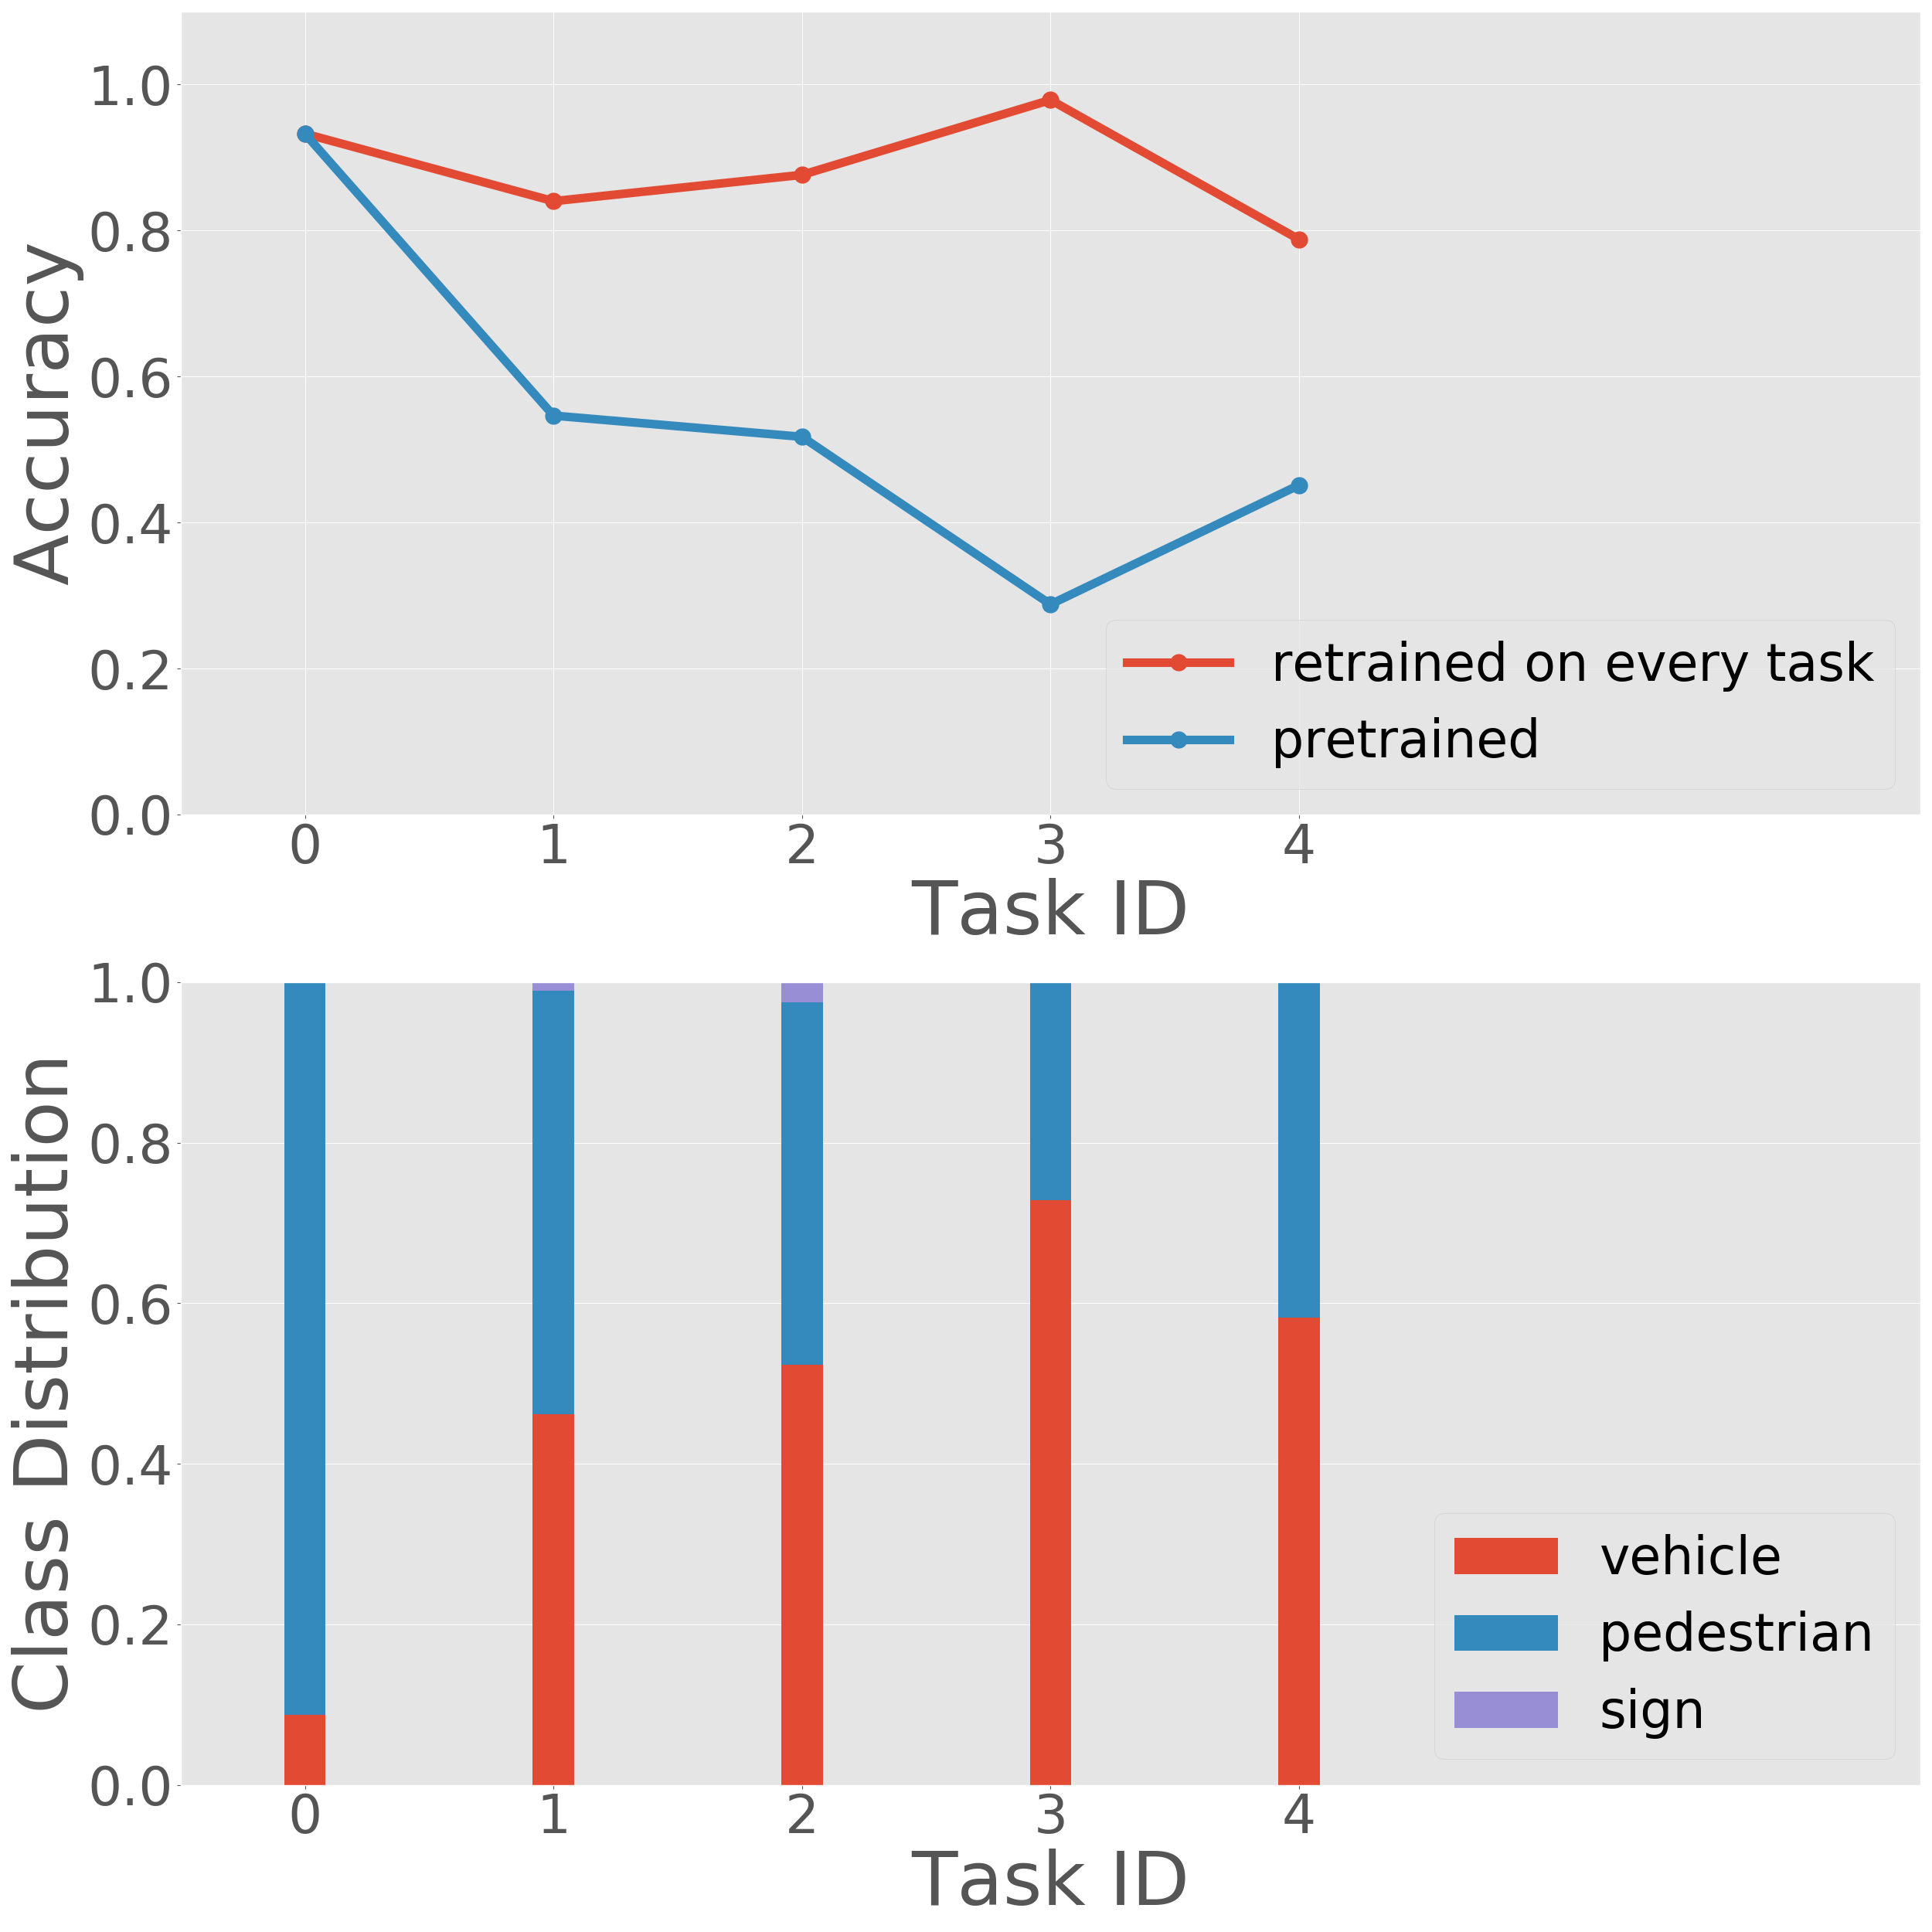
\includegraphics[width=\linewidth]{ekya/figures/motivation/Class_Incrementality/class_distribution_change_sf_27.png}
%     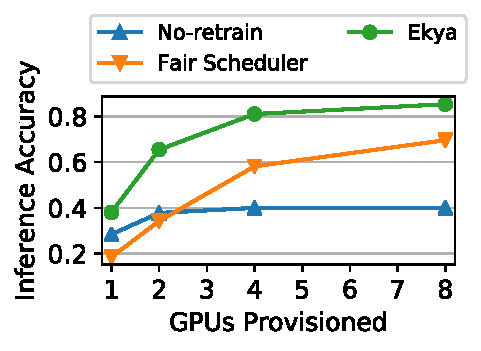
\includegraphics[width=\linewidth]{results/multicam/multicam_acc_vs_res_waymo.pdf}
%      \caption{\small Waymo}
%     \label{fig:scalability-gpus-waymo}
%   \end{subfigure}
%   \begin{subfigure}[t]{0.3\linewidth}
%     \centering
%     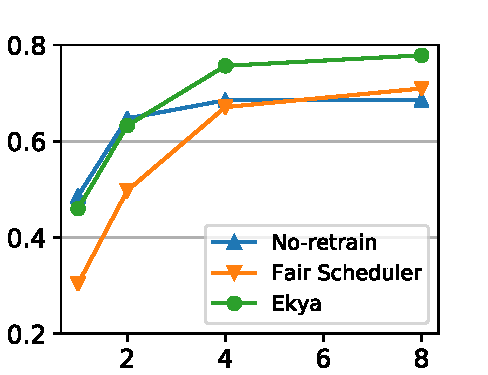
\includegraphics[width=\linewidth]{results/multicam/cityscapes_across_resources.pdf} 
%     \caption{\small Cityscapes}
%     \label{fig:scalability-gpus-cityscapes-golden}
%   \end{subfigure}
%   ~~~
%   \begin{subfigure}[t]{0.3\linewidth}
%     \centering
%     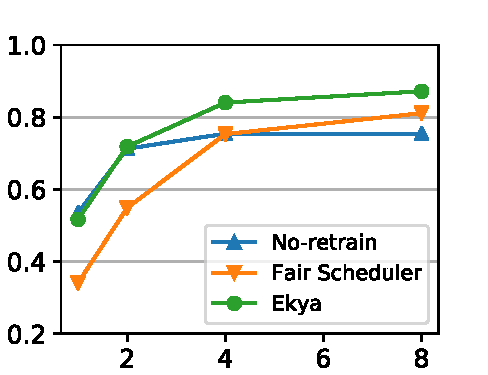
\includegraphics[width=\linewidth]{results/multicam/waymo_across_resources.pdf} 
%     \caption{\small Waymo}
%     \label{fig:scalability-gpus-waymo-golden}
%   \end{subfigure}
%   ~~~
%   \begin{subfigure}[t]{0.3\linewidth}
%     \centering
%     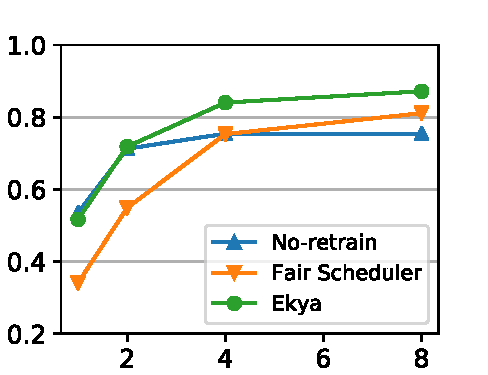
\includegraphics[width=\linewidth]{results/multicam/waymo_across_resources.pdf} 
%     \caption{\small \junchen{long video?}}
%     \label{fig:scalability-gpus-waymo-golden}
%   \end{subfigure}
  \begin{subfigure}[t]{0.47\linewidth}
    \centering
    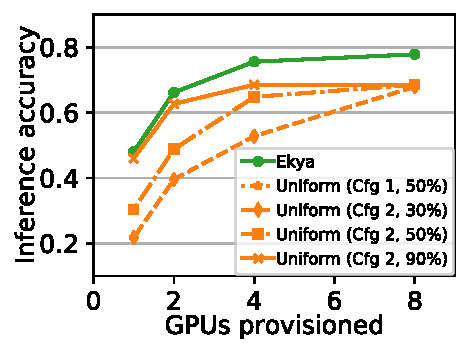
\includegraphics[width=\linewidth]{ekya/results/multicam/cityscapes_scheduler_comparison_across_resources.pdf}
    \caption{\small Cityscapes}
    \label{fig:scalability-gpus-cityscapes-golden}
  \end{subfigure}
  ~~~
  \begin{subfigure}[t]{0.47\linewidth}
    \centering
    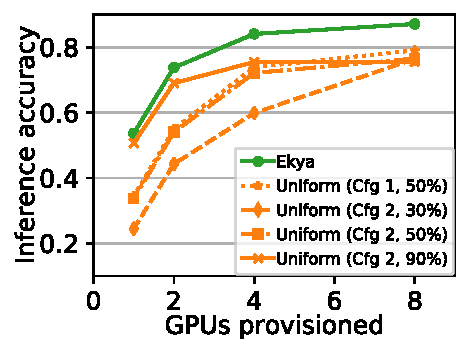
\includegraphics[width=\linewidth]{ekya/results/multicam/waymo_scheduler_comparison_across_resources.pdf} 
    \caption{\small Waymo}
    \label{fig:scalability-gpus-waymo-golden}
  \end{subfigure}
  \\
  \begin{subfigure}[t]{0.47\linewidth}
    \centering
    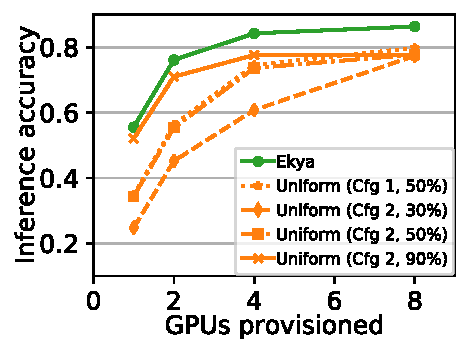
\includegraphics[width=\linewidth]{ekya/results/multicam/las_vegas_scheduler_comparison_across_resources.pdf} 
    \caption{\small Urban Building}
    \label{fig:scalability-gpus-lasvegas-golden}
  \end{subfigure}
  ~~~
  \begin{subfigure}[t]{0.47\linewidth}
    \centering
    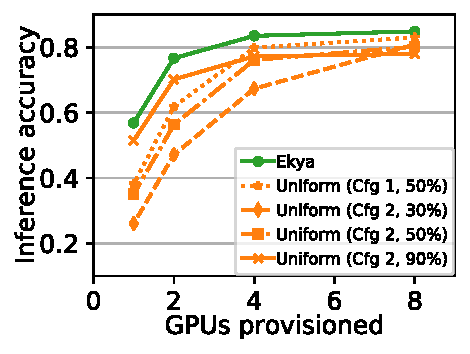
\includegraphics[width=\linewidth]{ekya/results/multicam/bellevue_10cam_scheduler_comparison_across_resources.pdf} 
    \caption{\small Urban Traffic}
    \label{fig:scalability-gpus-bellevue-golden}
  \end{subfigure}
  \caption{\small \bf Inference accuracy of different schedulers when processing 10 video streams under varying GPU provisionings.
  }
  \label{fig:scalability-gpus}
\end{figure}


% \junchen{once Romil generates the implementation results, will change the order to put impl-based graphs first and move accuracy vs resource to after that.}
\mypara{Accuracy vs. provisioned resource}
Finally, Figure~\ref{fig:scalability-gpus} stress-tests \name and the \fair baselines to process 10 concurrent video streams and shows their average inference accuracy under different number of GPUs. 
% , with the \fair baselines under various retraining configurations and resource partitionings.
To scale to more GPUs, we use the simulator (\S\ref{subsec:eval-setup}), which uses profiles recorded from real tests and we verified that it produced similar results as the implementation at small-scale.
% In each of the Waymo and Cityscapes traces, we randomly pick 10 video streams and run their inference concurrently through five retraining windows.
As we increase the number of provisioned GPUs, we see that \name consistently outperforms the best of the two baselines by a considerable margin and more importantly, with 4 GPUs \name achieves higher accuracy (marked with the dotted horizontal line) than the baselines at 16 GPUs (\ie 4$\times$ resource saving).


%\revtext{The above results highlight \name's operating regime: \name is more beneficial when the resources on the edge are oversubscribed (\ie there are more jobs than resources). This oversubscription creates an opportunity for \name's scheduler to intelligently reallocate resources to jobs which can benefit more from the same resources. Oversubscription is common in edge settings, since unlike cloud services, the amount of resources provisioned at the edge is carefully set to fit the workloads of individual edge nodes and minimize idle resources.}
\revtext{The above results show that \name is more beneficial when there is high contention for the GPU on the edge. %Such contention creates the opportunity for \name's scheduler to intelligently allocate resources. % to jobs that benefit more from the allocated resources. 
Under low contention, the room for improvement shrinks. %However, unlike 
Contention is, however, common in the edge since the resources are tightly provisioned to minimize their idling.
}

% In situations when resources are underutilized, it is possible to allocate excess resources to retraining without hampering inference performance, which nullifies the need for a scheduling system like \name. However, these under-utilization situations are unlikely since the amount of resources provisioned at the edge is carefully set to minimize idle resources.

% \revtext{As seen here, the benefits of using Ekya are best demonstrated when the resources on the edge are oversubscribed, i.e. there are more jobs than resources. This oversubscription creates an opportunity to intelligently reallocate resources to jobs which can benefit more from the same resources. In situations when resources are underutilized, it is possible to allocate excess resources to retraining without hampering inference performance, which nullifies the need for a scheduling system like \name. However, these under-utilization situations are unlikely since the amount of resources provisioned at the edge is carefully set to minimize idle resources.}

% ---\fillme-\fillme\% higher accuracy in Cityscapes, \fillme-\fillme\% in Waymo, and  \fillme-\fillme\% in the long traffic video.

% While accuracy gap between \name{} and the \fair baseline decreases as more GPUs are provisioned, \name needs much less resources---upto $\fillme\times$ less GPUs---to achieve the maximum accuracy that \fair scheduler attains with 8 GPUs.



% (where \name achieves an average inference accuracy of 0.78.

%Figure~\ref{fig:history-vs-current} compares 
% We compare the accuracy of retraining the model on the current window (\name) with the accuracy of re-using the model from a history window in which the class distribution is the closest to the distribution in the current window in terms of their Euclidean distance. \junchen{check it with Zhengxu/Romil}
% % (Euclidean distance $\leq 0.2$; \S\ref{sec:profiling}). 
% Here we use ResNet18 as the model and Waymo as the trace (the findings are similar for other models and datasets).
% %The graph, however, shows 
% We observe that 
% the accuracy is much lower by re-using the model from history, even when the history window share a similar class distribution. At median, the difference in accuracy is 11\% with the $90^\text{th}$ percentile and maximum divergence in accuracies being as high as $38\%$ and $51\%$.
% This confirms our intuition in \S\ref{sec:profiling} that although sharing a similar class distribution is indicative of the difficulty of retraining, it does not mean the model can be directly reused from any window with similar class distribution. \junchen{is this intuition mentioned anywhere any more?}

% \mypara{Summary}
% The results highlight three properties of \name. 
% First, it allocates resources to retraining only when the accuracy gain from the retraining outweighs the temporary inference accuracy drop due to frame subsampling.
% Second, when it allocates resource to retraining, it retrains the model with a configuration that can finish in time for the inference to leverage the higher accuracy from the retrained model.
% \revtext{Finally, \name's benefits generalize to different ML tasks (of classification and detection) across many model architectures.}% which explains why \name outperforms the no-retraining baseline. 
% Being able to adapt both configuration and resource allocation allows \name to optimally leverage the edge resource and thus outperform both edge-based baselines as well as the cloud-based baseline and the reusing-pretrained-model baseline.
% Moreover, when \name allocates resource to retraining, it allocates minimum amount needed by the retraining to finish in time, thus outperforming the fair scheduler.


% \end{packeditemize}

%\begin{figure}[t!]
%\centering
%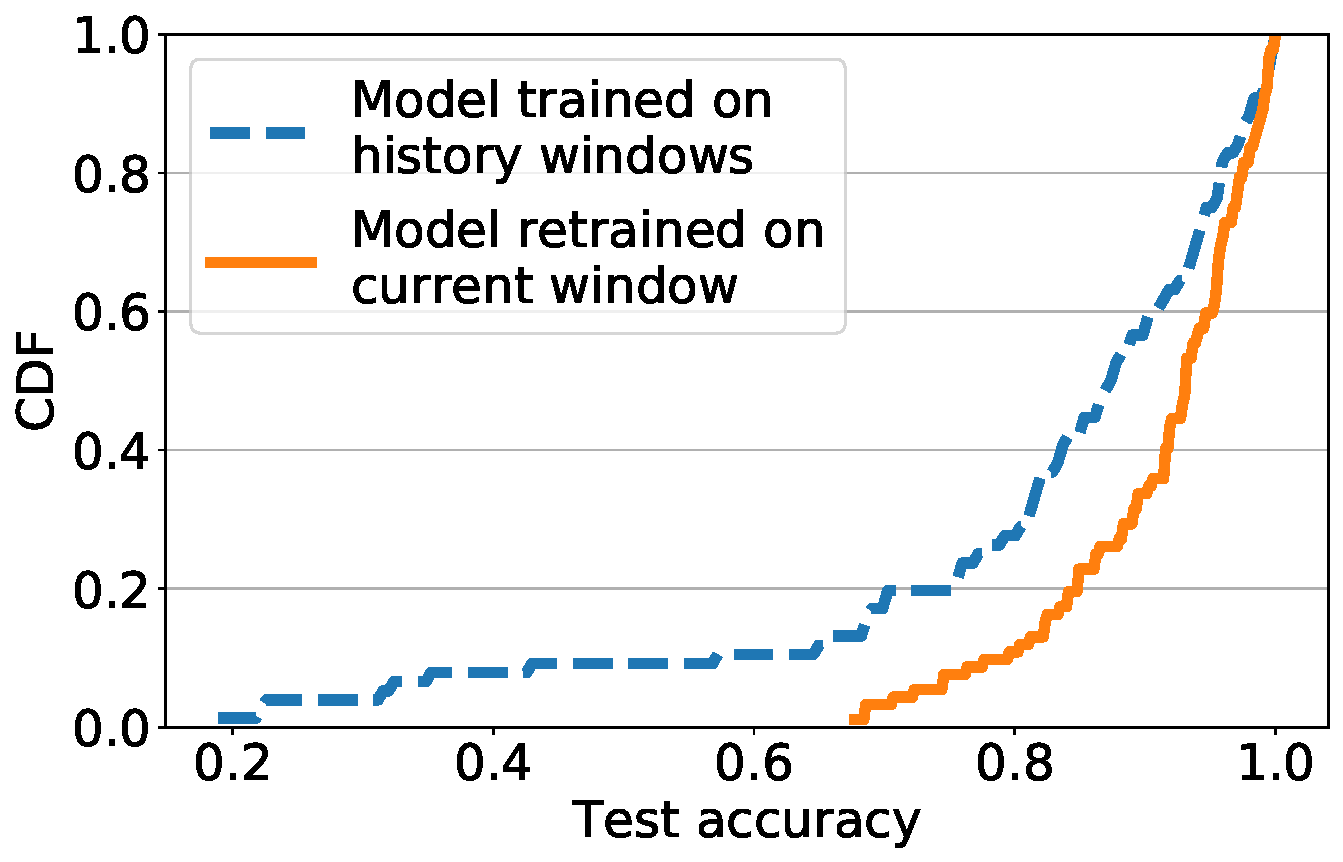
\includegraphics[width=0.6\columnwidth]{ekya/figures/eval_placeholders/history-trained-vs-retrained-cdf.pdf}
%\vspace{-0.2cm}
%\caption{\bf\small Gap between accuracy of the model retrained in the current and accuracy of re-using a model retrained in a history window that share similar class distribution.
%\vspace{-0.2cm}}
%\label{fig:history-vs-current}
%\end{figure}



% Math sheet- https://docs.google.com/spreadsheets/d/1z4Zui8Qmg4iH-_yQKu7p0EZtXOlj_-ogKIW9mbf-Tpo/edit#gid=179811194

% For instance, each retraining window in the Waymo dataset accumulates about 1760 Mb of data every 20 seconds, resulting in a 88 Mb/s bitrate. Assuming a 10\% sub-sampling rate for retraining and a retraining window of 200 seconds (as in all our experiments), a total of 1760 Mb  of training data must be sent to the cloud. With an uplink of 5.1 Mb/s \cite{opensignal_2018}, just uploading the training data would take 345 seconds. Moreover, the updated model weights need to be downloaded from the cloud, which is 360 Mb in size. With a downlink throughput of 17.3 Mb/s \cite{opensignal_2018} (cellular connection), that adds another 20 seconds. Combined, this results in nearly 365s to get the retrained model, which far exceeds the retraining window size of 5 minutes (note that we have ignored the time to run the training in the cloud). Since even the sub-sampled video bitrate exceeds the limited bandwidths at the edge, this analysis applies for all retraining window sizes.





% 6.3 Understanding Ekya improvements

% - ablation analysis

% - per-stream gains

% - temporal behaviors

\subsection{Understanding Ekya's improvements}
\label{subsec:eval-understanding}

\begin{figure}
\captionsetup[subfigure]{justification=centering}
  \centering
  \begin{subfigure}[t]{0.45\linewidth}
    \centering
    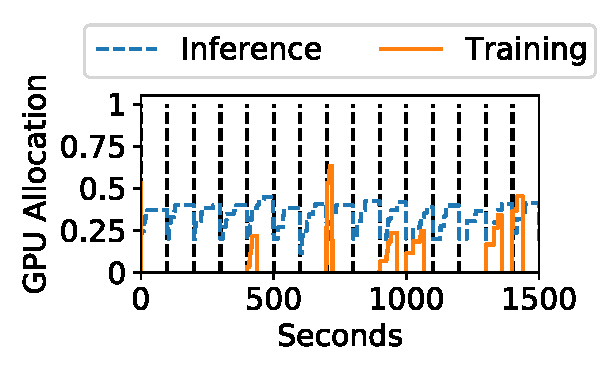
\includegraphics[width=\linewidth]{ekya/results/multicam/long_video_gpu_allocation_vs_time_cam1.pdf}
    \caption{\small Video stream \#1 \\(Inference accuracy = 0.82)}
    \label{fig:temporal-video-1}
  \end{subfigure}
  ~
  \begin{subfigure}[t]{0.45\linewidth}
    \centering
    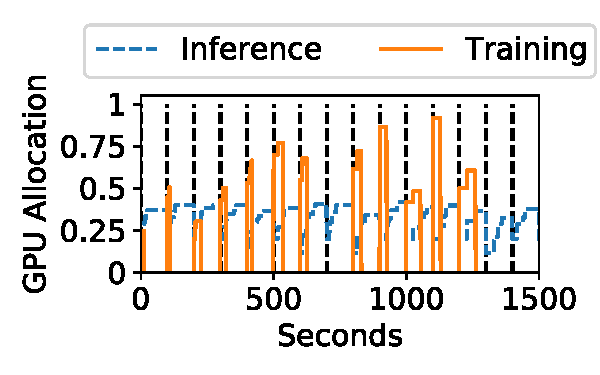
\includegraphics[width=\linewidth]{ekya/results/multicam/long_video_gpu_allocation_vs_time_cam5.pdf} 
    \caption{\small Video stream \#2 \\(Inference accuracy = 0.83)}
    \label{fig:temporal-video-2}
  \end{subfigure}
  \caption{\small \bf \name's resource allocation to two video streams over time. \name adapts when to retrain each stream's model and allocates resource based on the retraining benefit to each stream.}
  \label{fig:temporal-resource-allocation}
\end{figure}

% \begin{figure} [t!]
%  	%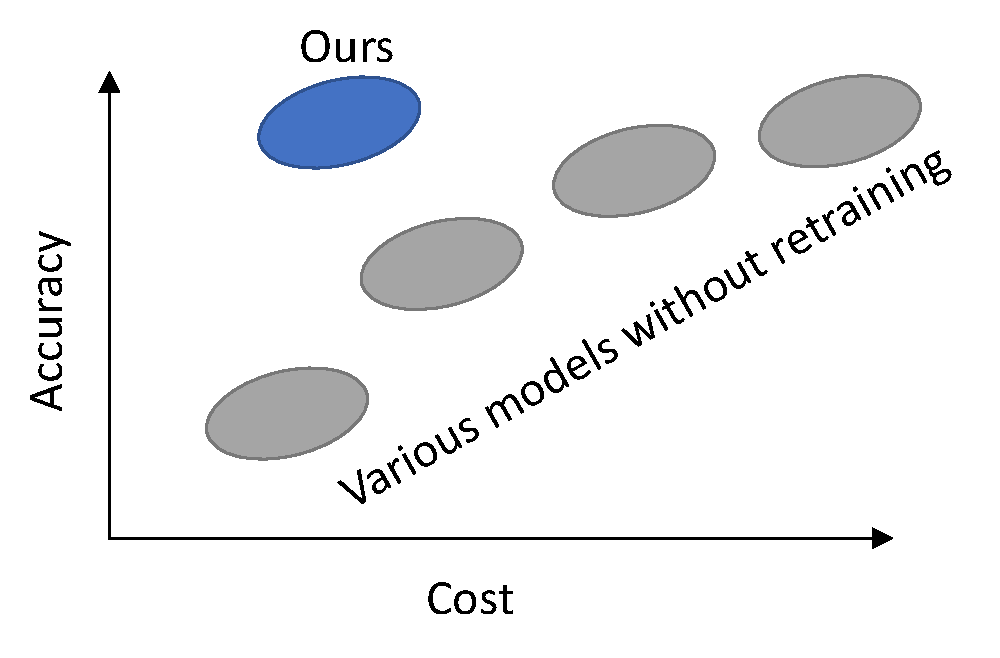
\includegraphics[width=0.4\textwidth]{ekya/figures/eval_placeholders/single-tradeoffs.pdf}
%  	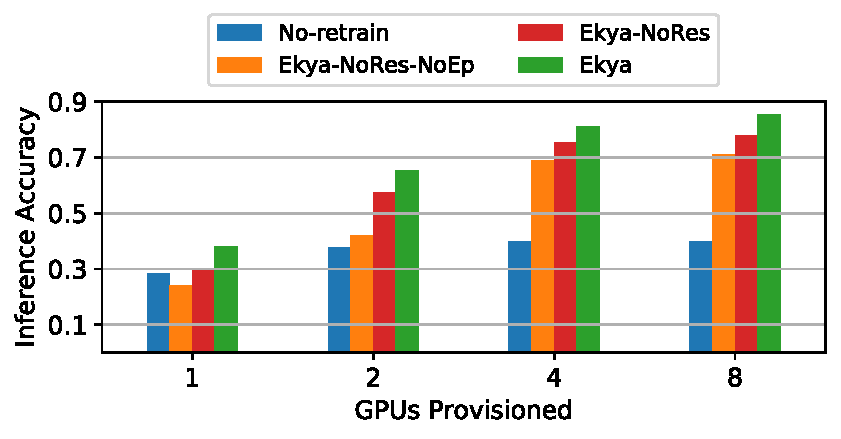
\includegraphics[width=\linewidth]{results/ablation_waymo.pdf}
% 	\caption{\small \bf {\name} factor analysis by removing  dynamic resource allocation and reducing the hyperparameter space.}
% 	\label{fig:factor-analysis}
% \end{figure}

\mypara{Resource allocation across streams}
Figure~\ref{fig:temporal-resource-allocation} shows \name's resource allocation across two example video streams over several retraining windows. 
In contrast to the \fair baselines that use the same retraining configuration and allocate equal resource to retraining and inference (when retraining takes place), \name retrains the model only when it benefits and allocates different amounts of GPUs to the retraining jobs of video streams, depending on how much accuracy gain is expected from retraining on each stream. 
In this case, more resource is diverted to video stream \#1 (\#1 can benefit more from retraining than \#2) and both video streams achieve much higher accuracies (0.82 and 0.83) than the \fair baseline.
% , which suggests that the resources are allocated based on the relative gains between retraining and inference.
% \romil{1) Are the accuracy numbers relevant here? 2) We should note that inference accuracies increase as training jobs in a window complete. }

\mypara{Component-wise contribution}
% improvement breakdown
% \mypara{Factor analysis}
Figure~\ref{fig:factor-analysis} understands the contributions of resource allocation and configuration selection (on 10 video streams with 4 GPUs provisioned). 
% To understand the contribution of each part of \name, we run a factor analysis on the same setting as  
We construct two variants from {\name}:
\emph{Ekya-FixedRes}, which removes the smart resource allocation in \name (\ie using the inference/training resource partition of the \fair baseline), 
and \emph{Ekya-FixedConfig} removes the microprofiling-based configuration selection in \name (\ie using the fixed configuration of the \fair baseline). 
Figure~\ref{fig:factor-analysis} shows that both adaptive resource allocation and configuration selection has a substantial contribution to \name{}'s gains in accuracy, especially when constrained (i.e., fewer resources are provisioned). 
% On the other hand, with more resources, even expensive retraining configurations can be applied, thus configuration selection matters less. The smart resource allocation mechanism in {\name} has a nearly consistent contribution to \name{}'s performance. 
% \junchen{needs to update once Figure~\ref{fig:scalability-gpus} is updated!}
% and additionally fixes the number of epochs a model is trained to the maximum value, effectively removing it from the configuration space. 
% We chose this hyperparameter for removal because it creates the largest diversity in the resource-accuracy profiles of configurations. 

% \emph{Ekya-NoRes}, which removes the smart resource allocation in \name. \emph{Ekya-NoRes-NoEp} removes resource allocation and additionally fixes the number of epochs a model is trained to the maximum value, effectively removing it from the configuration space. We chose this hyperparameter for removal because it creates the largest diversity in the resource-accuracy profiles of configurations. 

% As observed in Figure \ref{fig:factor-analysis}, the diversity in configurations and their careful selection has a large contribution to \name{}'s gains in accuracy when fewer resources are provisioned, which reduces as more resources are made available. This is because with more resources, even expensive configurations become feasible, thus configuration selection matters less. The smart resource allocation mechanism in {\name} has a nearly consistent contribution to \name{}'s performance.

%We note that the accuracy of \emph{Ekya-NoRes-NoEp} is lower than \emph{No-retrain} when 1 GPU is provisioned because resource reallocation is removed, and thus it always allocates resources to retraining. It just so happens that there are no good configurations to pick from once the epochs hyperparameter is removed, and thus the accuracy is lesser than \emph{No-retrain}.


% \begin{figure} [t!]
%  	%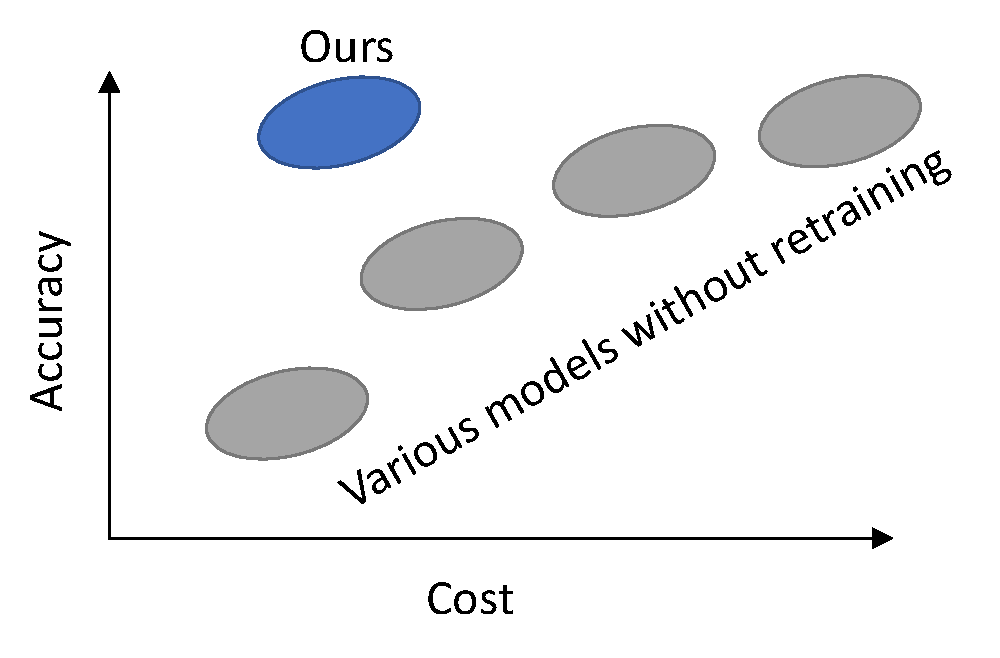
\includegraphics[width=0.4\textwidth]{ekya/figures/eval_placeholders/single-tradeoffs.pdf}
%  	\includegraphics[width=0.85\linewidth]{results/ablation_cityscapes_2.pdf}
% 	\caption{\small \bf A factor analysis of \name that shows the impact of removing dynamic resource allocation (Ekya-FixedRes) or removing retraining configuration adaptation (Ekya-FixedConfig). 
% % 	\romil{Nit: Legend textures are not clear, can reduce legend font size by a bit to avoid overlapping the ylabel} 
% % 	\junchen{this should be \fair => \name (w/o config adaptation) => \name (w/o resource allocation) => \name. needs to update!}
% 	}
% 	\label{fig:factor-analysis}
% \end{figure}




\revtext{
\mypara{Retraining window sensitivity analysis}
% \begin{figure} [t!]
%  	\includegraphics[width=0.9\linewidth]{results/sensitivity/retraining_window_sensitivity.pdf}
% 	\caption{\small \bf A sensitivity analysis of the retraining window parameter. \name is robust to a wide range of retraining window values and gracefully degrades to an accuracy equivalent of no retraining if the window size is too small. If the window size is too large, the model's generalizability becomes the limiting factor, slowly reducing the accuracy as more training data accumulates.
% 	}
% 	\label{fig:window-sensititvity}
% \end{figure}
Figure~\ref{fig:window-sensititvity} evaluates the sensitivity of \name to the retraining window size. %, which governs how frequently a model will be retrained. %We also compare a no-retraining baseline where a pre-trained model is used without any continuous retraining.
\name is robust to different retraining window sizes. When the retraining window size is too small (10 seconds), the accuracy of \name is equivalent to no retraining accuracy due to insufficient time and resources for retraining. As the window increases, \name's performance quickly ramps up because the thief scheduler is able to allocate resources to retraining. As the retraining window size further increases Ekya's performance slowly starts moderately degrading because of the inherent limitation in capacity of compressed models (\S\ref{subsec:continuous-measurement}). %Note that this degradation is a consequence of the using compressed models and can be avoided by using a larger model.
}



\mypara{Impact of scheduling granularity}
% sensitivity to granularity
% \mypara{Sensitivity to scheduling granularity} 
% \ga{Change $\delta$ to $\Delta$ in the graphs and text.}
A key parameter in \name's scheduling algorithm (\S\ref{subsec:thief}) is the allocation quantum $\Delta$: it controls the runtime of the scheduling algorithm and the granularity of resource allocation.
%Figure~\ref{fig:sensitivity-delta} plots this tradeoff with the same setting as Figure~\ref{fig:scalability-gpus} (10 video streams). % with 4 or 8 GPUs provisioned).
In our sensitivity analysis with 10 video streams, we see that 
%While 
increasing $\Delta$ from $1.0$ (coarse-grained; one full GPU) to $0.1$ (fine-grained; fraction of a GPU), increases the accuracy substantially by $\sim8\%$. %we see the accuracy increases substantially $\sim8\%$.
Though the runtime also increases to 9.5 seconds, it is still a tiny fraction ($4.7\%$) of the retraining window ($200$s).%, and hence we use $\Delta=0.1$ in our experiments.
% Between $\Delta=0.1$ and $1.0$, higher $\delta$ reduces the runtime of the scheduler by 4$\times$, but the accuracy gain is severely affected. 
% One should pick a higher $\Delta$ only when the scheduler is relatively slow compared to a retraining window; 
% otherwise, a low value of $\Delta$ (fine-grained scheduling) is preferable.
% \junchen{highlight the runtime is low}


% \begin{figure}
%   \centering
%   \begin{subfigure}[t]{\linewidth}
%     \centering
%     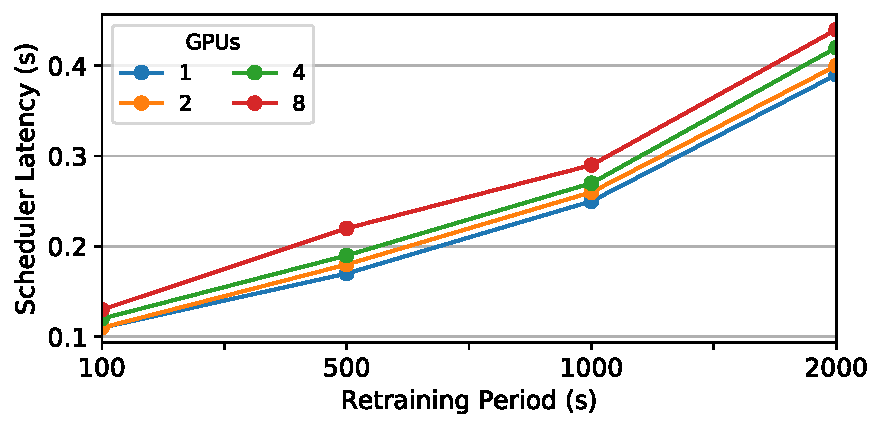
\includegraphics[width=\linewidth]{results/sensitivity/scheduler_resourcetime.pdf}
%   \end{subfigure}
%   \caption{\small \bf Thief scheduler latency for scheduling 10 video streams with varying available resource quantities and retraining period durations. The scheduler latency is a tiny fraction compared to the duration of the retraining period.  }
%   \label{fig:sensitivity-schedlatency}
% \end{figure}

%%%\begin{figure}
%%%  \centering
%%%  \begin{subfigure}[t]{0.95\linewidth}
%%%\centering
%%%    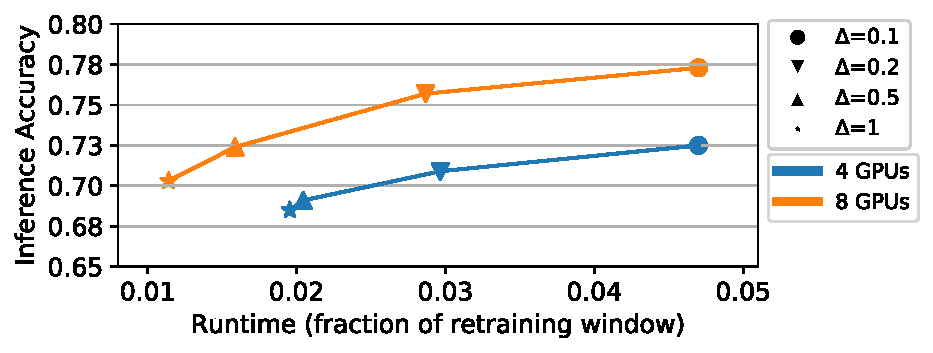
\includegraphics[width=\linewidth]{results/sensitivity/sensitivity_delta_acc_runtime_cityscapes_48gpu.pdf}
%%%  \end{subfigure}
%%%  \caption{\small \bf {Effect of the $\Delta$ parameter on the thief scheduler. Smaller values increase the runtime (though still a tiny fraction of a retraining window of 200s) but improve the accuracy.}}
%%%  \label{fig:sensitivity-delta}
%%%\end{figure}

% Sys Impl result
\begin{figure}
\captionsetup[subfigure]{justification=centering}
  \centering
  \begin{subfigure}[t]{0.45\linewidth}
    \centering
    \includegraphics[width=\linewidth]{ekya/results/ablation_cityscapes_2.pdf}
    \caption{\small Factor analysis}
    \label{fig:factor-analysis}
  \end{subfigure}
  \begin{subfigure}[t]{0.48\linewidth}
    \centering
    \includegraphics[width=\linewidth]{ekya/results/sensitivity/retraining_window_sensitivity.pdf}
    \caption{\small\revtext{Sensitivity to retraining window size.}}
    \label{fig:window-sensititvity}
  \end{subfigure}
  ~~~
  \caption{\revtext{\small \bf (a) Component-wise impact of removing dynamic resource allocation (50\% allocation) or removing retraining configuration adaptation (fixed Cfg 2). (b) Robustness of \name to a wide range of retraining window values.% and a graceful degradation to the baseline when retraining is infeasible.
  }
  }
  \label{fig:factor-sensisitvity-group}
\end{figure}




\subsection{Effectiveness of micro-profiling}
\label{subsec:eval-profiling}


\begin{figure}[t]
\captionsetup[subfigure]{justification=centering}
  \centering
  \begin{subfigure}[t]{0.48\linewidth}
    \centering
    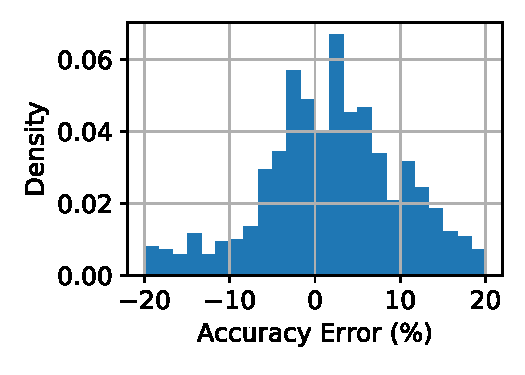
\includegraphics[width=\linewidth]{ekya/results/microprofiling/microprofiling_accerror.pdf}
    \caption{\small Distribution of accuracy estimation errors.}
    \label{fig:microprofiling-benchmark}
  \end{subfigure}
  ~
  \begin{subfigure}[t]{0.48\linewidth}
    \centering
    \includegraphics[width=\linewidth]{ekya/results/sensitivity/sensitivity_profileerrors_cityscapes.pdf} 
    \caption{\small Impact of an controlled error $\epsilon$ to accuracy estimates.}
    \label{fig:sensitivity-accuracy-error}
  \end{subfigure}
  \caption{
      \small \bf Evaluation of microprofiling performance. (a) shows the distribution of microprofiling's actual estimation errors, and (b) shows the robustness of \name's performance against microprofiling's estimation errors.
  }
%   \label{fig:temporal-resource-allocation}
\end{figure}


\revtext{The absolute cost of micro-profiling is small; for our experiments, micro-profiling takes 4.4 seconds for a 200s window. %This cost can be changed by reducing or increasing the configurations to be explored.
}

\mypara{Errors of microprofiled accuracy estimates}
\name's micro-profiler estimates the accuracy of each configuration (\S\ref{subsec:profiling}) by training it on a subset of the data for a small number of epochs. 
To evaluate the micro-profiler's estimates, we run it on all configurations for 5 epochs and on 10\% of the retraining data from all streams of the Cityscapes dataset, and calculate the estimation error against the retrained accuracies when trained on 100\% of the data for 5, 15 and 30 epochs. 
% \junchen{can we just focus on 30 epochs?}
Figure~\ref{fig:microprofiling-benchmark} plots the distribution of the errors in accuracy estimation and and show that the micro-profiled estimates are largely unbiased with an median absolute error of 5.8\%. % Mean was 8.7%

% Ekya relies on a micro-profiler to estimate the accuracy of configurations (\S\ref{subsec:profiling}) by training it on a subset of the training data for a small number of epochs. To evaluate the accuracy predictions from the micro-profiler, we run the microprofiler for 5 epochs and on 10\% of the data for each retraining window for 10 cities in the Cityscapes dataset and use it to predict the accuracies when the configuration is trained on 100\% of the data for 5, 15 and 30 epochs. \cref{fig:microprofiling-benchmark} plots a probability distribution of the error in accuracy estimation from microprofiling. Micro-profiling produces unbiased estimates with an median absolute \% error of 5.8\%. % Mean was 8.7%

% \begin{table}[]
% \footnotesize
% \begin{tabular}{cccc}
% \toprule
% \textbf{Network} & \textbf{\begin{tabular}[c]{@{}c@{}}Uplink\\ (Mbps)\end{tabular}} & \textbf{\begin{tabular}[c]{@{}c@{}}Downlink\\ (Mbps)\end{tabular}} & \textbf{Accuracy} \\ \midrule
% Cellular 4G      & 5.1             & 17.5              & 68.5\%            \\ \midrule
% Satellite        & 8.5             & 15                & 69.2\%            \\ \midrule
% Cellular 4G x2   & 10.2              & 35                & 71.2\%            \\ \midrule
% % Cable            & 19.5            & 99                & 75.8\%            \\ \midrule 
% % Fiber            & 50.5            & 67                & 77.7\%            \\ \midrule
% \textbf{{\name}}             & -               & -                 & \textbf{77.8\%}          \\
% \bottomrule
% \end{tabular}
% \caption{\label{tab:cloudexpt}\small\bf Training in the cloud with varying network capacities~\cite{edgelandscape} versus using {\name} at the edge.  {\name} delivers retrained models faster than the upload-download delay of modern edge network links, achieving a higher accuracy.}
% \end{table}


% \begin{table}[]
% \footnotesize
% \begin{tabular}{ccccc}
% \toprule
% \textbf{Network} & \textbf{\begin{tabular}[c]{@{}c@{}}Uplink/Downlink\\ (Mbps)\end{tabular}} & \textbf{Accuracy} & \textbf{\begin{tabular}[c]{@{}c@{}}Additional Bandwidth \\ (Uplink/Downlink)\end{tabular}} \\ \midrule
% Cellular 4G      & 5.1/17.5               & 68.5\%     &     3.8x/10.2x       \\ \midrule
% Satellite        & 8.5/15               & 69.2\%       &     3.8x/10.2x       \\ \midrule
% % Cellular 4G x2   & 10.235              & 35                & 71.2\%            \\ \midrule
% % Cable            & 19.5            & 99                & 75.8\%            \\ \midrule 
% % Fiber            & 50.5            & 67                & 77.7\%            \\ \midrule
% \textbf{{\name}}             & -/-                     & \textbf{77.8\%}     &     -/-     \\
% \bottomrule
% \end{tabular}
% \caption{\label{tab:cloudexpt}\small\bf Training in the cloud with varying network capacities~\cite{edgelandscape} versus using {\name} at the edge.  {\name} delivers retrained models faster than the upload-download delay of modern edge network links, achieving a higher accuracy.}
% \end{table}

\begin{table}[t]
\footnotesize
% \begin{tabular}{ccccc}
% \hline
% \multirow{2}{*}{{\bf Network}} & \multirow{2}{*}{\begin{tabular}[c]{@{}c@{}}{\bf Uplink/Downlink}\\ (Mbps)\end{tabular}} & \multirow{2}{*}{{\bf Accuracy}} & \multicolumn{2}{c}{{\bf Add. bandwidth needed}} \\ \cline{4-5} 
%  &  &  & Uplink & Downlink \\ \hline
% Cellular 4G & 5.1/17.5 & 68.5\% & 3.8x & 10.2x \\ \hline
% Satellite & 8.5/15 & 69.2\% & 3.8x & 10.2x \\ \hline
% \textbf{{\name}}  & -/- & {\bf 77.8\%} & 0 & 0 \\ \hline
% \end{tabular}
\begin{tabular}{cccccc}
\hline
\multirow{2}{*}{} & \multicolumn{2}{c}{Bandwidth (Mbps)} & \multirow{2}{*}{Acc.} & \multicolumn{2}{c}{Bandwidth Gap} \\ \cline{2-3} \cline{5-6} 
 & Uplink & Downlink &  & Uplink & Downlink \\ \hline
Cellular & 5.1 & 17.5 & 68.5\% & 10.2$\times$ & 3.8$\times$ \\ \hline
Satellite & 8.5 & 15 & 69.2\% & 5.9$\times$ & 4.4$\times$ \\ \hline
Cellular ($2\times$) & 10.2 & 35 & 71.2\% & 5.1$\times$ & 1.9$\times$ \\ \hline
% Cellular ($2\times$) & 5.1 & 17.5 & 68.5\% & 3.8$\times$ & 10.2$\times$ \\ \hline
{\bf \name} & - & - & {\bf 77.8\%} & {\bf -} & {\bf -} \\ \hline
\end{tabular}
\caption{\label{tab:cloudexpt}\small\bf Retraining in the cloud under different networks~\cite{39-getmobile, 57-getmobile, getmobile} versus using {\name} at the edge. \name achieves better accuracy without using expensive satellite and cellular links. 
%{\name} delivers retrained models faster than the upload-download delay of modern edge network links, achieving a higher accuracy. %\junchen{needs to update the satellite row}
}
\end{table}



\mypara{Sensitivity to microprofiling estimation errors}
% sensivity to accuracy errors
% \mypara{Sensitivity to accuracy estimation errors}
%Resource consumption and accuracy of accuracy estimation. E
Finally, we test the impact of accuracy estimation errors (\S\ref{subsec:profiling}) on \name.
We add gaussian noise on top of the predicted retraining accuracy when the microprofiler is queried. 
Figure~\ref{fig:sensitivity-accuracy-error} shows that \name is robust to accuracy estimate errors: with upto 20\% error (which covers all errors in Figure~\ref{fig:microprofiling-benchmark}) in the profiler prediction, the maximum accuracy drop is 3\%. 
% Even when a 50\% profiling error is introduced, the accuracy drop is 7.9\% points. Such a large profiling error makes \name{} worse than the no-retrain baseline, but still better than fair scheduling.

% We now test the impact of errors of accuracy estimates (\S\ref{subsec:profiling}) on \name's overall performance.
% To control the amount of errors, we add a controlled Gaussian noise on top of the real retraining accuracy as the predictions when the profiler is queried. 
% Figure~\ref{fig:sensitivity-accuracy-error} shows that with upto 20\% errors in the profiler prediction, the maximum accuracy drop is 3\% points. When a 50\% profiling error is introduced, the accuracy drop is 7.9\% points. Such a large profiling error makes \name{} worse than the no-retrain baseline, but still better than fair scheduling.

% \begin{figure}
% 	\includegraphics[width=\linewidth]{results/sensitivity/sensitivity_profileerrors_cityscapes.pdf}
% 	\caption{\small \bf Adding a controlled error $\epsilon$ to the accuracy prediction -  \name{}'s performance degrades, but only marginally.}
% 	\label{fig:sensitivity-accuracy-error}
% \end{figure}







% \subsection{Ekya vs  baselines}
\subsection{Comparison with alternative designs}
\label{subsec:eval-alternate}
%We evaluate alternatives to continuous retraining on the edge.
% ---(1) re-using a retrained model from a history window that shares class distribution (instead of retraining the model again) and (2) offloading the retraining to the cloud.

\mypara{Ekya vs. Cloud-based retraining}
One may upload a sub-sampled video stream to the cloud, retrain the model, and download the model back to the edge~\cite{khani2020real}. %(the workflow is similar to a recent work~\cite{khani2020real}).
While this solution is not an option for many deployments due to legal and privacy stipulations \cite{sweden-data, azure-data}, we still evaluate this option as it lets the edge servers focus on inference. Cloud-based solutions, however, results in lower accuracy due to significant network delays %the delay of uploading the training data and downloading the retrained models 
on the constrained networks typical of edges \cite{getmobile}.
%It is fundamentally challenging to run continuous learning across the edge-cloud because of network constraints.
% Math sheet new - https://docs.google.com/spreadsheets/d/1-WDeFmQwHy0sEpxL9f6QcbMKt1DVPaX6ODjMwDbb3IY/edit#gid=0

For example, consider 8 video streams running ResNet18 and a retraining window of 400 seconds. 
A HD (720p) video stream at 4Mbps and 10\% data sub-sampling (typical in our experiments) amounts to 160Mb of training data per camera per window. 
Uploading 160Mb for each of the 8 cameras over a 4G uplink (5.1 Mbps \cite{57-getmobile}) and downloading the trained ResNet18 models (398 Mb each~\cite{torchvision-models}) over the 17.5 Mbps downlink \cite{57-getmobile} takes 432 seconds (even excluding the model retraining time), which already exceeds the retraining window.

To test on the Cityscapes dataset, we extend our simulator (\S\ref{subsec:eval-setup}) to account for network delays during retraining, and test with 8 videos and 4 GPUs. We use the conservative assumption that retraining in the cloud is ``instantaneous'' (cloud GPUs are powerful than edge GPUs). Table \ref{tab:cloudexpt} lists the accuracies with cellular 4G links (both one and two subscriptions to meet the 400s retraining window) and a satellite link, which are both indicative of edge deployments \cite{getmobile}. % We use two cellular links so as to meet the 400s retraining window (based on the description above). 

%{\name} achieves a higher accuracy of 77.8\% compared to the cloud alternatives. In fact, for 
For the cloud alternatives to match {\name}'s accuracy, we will need to provision additional uplink capacity of 5$\times$-10$\times$ and downlink capacity of 2$\times$-4$\times$ (of the already expensive links). In summary, {\name}'s edge-based solution is better than a cloud alternate for retraining in {\em both} accuracy and network usage (\name sends no data out of the edge), all while providing privacy for the videos. 
\revtext{However, when the edge-cloud network has sufficient bandwidth, e.g., in an enterprise that is provisioned with a private leased connection, then using the cloud to retrain the models can be a viable design choice.}
% \revtext{However, we note that if there is sufficient bandwidth available to the cloud, such as a fiber link in a indoor surveillance scenario, then using the cloud to retrain the models may be more effective.} %Further optimizations need to be devised for the cloud-based solution. 

%%Table~\ref{tab:cloudexpt} shows the accuracy of this cloud-based baseline, when a satellite network is used or when the cellular network throughput is doubled, and their accuracy is always much lower than \name's.
% Even on doubling the 4G cellular bandwidth, the total upload-download delay is 216 seconds and the edge server will not get the retrained model for more than half of the retraining window. This results in a mean inference accuracy of 69.2\% (Table \ref{tab:cloudexpt}).
%\name can finish retraining in 52 seconds and increases the mean inference accuracy to 77.8\%. Moreover, even before the retraining completes, it can checkpoint models so that the inference jobs can use the latest retrained model (\S\ref{sec:system}). If the cloud-based solution were to achieve the same accuracy of \name, the cellular 4G downlink bandwidth would have to be $3.8\times$ higher and uplink bandwidth $10.2\times$ higher.
% in our simulations and still operates under the assumption that the cloud can provision parallel resources instantly and trains instantly.   
% By the same token, offloading the inference completely to the server may take even more bandwidth and be more burdensome than offloading the model retraining only which send only subsampled images.
%Although the cloud-based solution might be further optimized, \name still has the unique advantage of keeping the retraining jobs local and scheduling them in a way that only minimally affects inference jobs.

%\junchen{how much more bandwidth is needed for the cloud to work?}

% \romil{Remove this para and fig?} Figure~\ref{fig:cloud-expt} compares the resulting inference accuracy of \name and the cloud-based baseline.
% We can see that \fillme.
% We observe qualitatively similar results under different settings.
% By the same token, offloading the inference completely to the server may take even more bandwidth and be more burdensome than offloading the model retraining only which send only subsampled images.
% Although the cloud-based solutions might be further optimized, \name still has the unique advantage keeping the retraining jobs local, as long as it schedules them in a way that only minimally affects inference jobs.


% Mention do we have to send everything to the cloud.

% \begin{figure}
%  	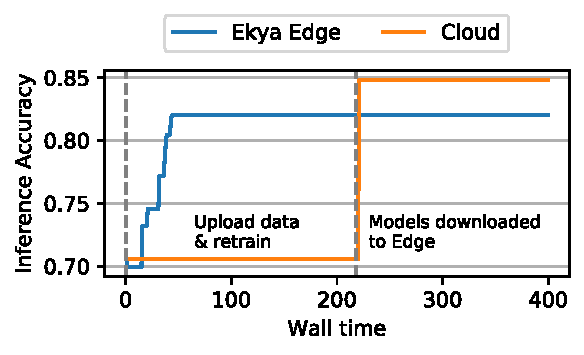
\includegraphics[width=0.8\linewidth]{results/cloud_expt.pdf}
% 	\caption{\small \bf Training in the cloud versus using Ekya at the edge. Ekya retrains faster and exploits models for longer. Training in the cloud requires expensive network transfers of data and models, which reduces the overall inference accuracy.}
% 	\label{fig:cloud-expt}
% \end{figure}


% % examples where the drop is higher
% Even on provisioning double the bandwidth (which entails an expensive change of the network link from cellular to cable), retraining on the cloud does not yield a higher accuracy in our simulator. We extend our simulator to simulate the network delays and assume that the the cloud offers a speed up of $10\times$ and has infinite parallel resources. Despite doubling the bandwidth, the delay introduced by the network results in a poor mean inference accuracy. 

% Figure \ref{fig:cloud-expt} demonstrates the effect of this delay for a retraining window. At time t=0, Ekya starts retraining at the edge while the cloud based solution starts uploading the training data to the cloud. The cloud \romilc{RTT}, which includes data upload, retraining and retrieving the models back to the edge takes 216 seconds, whereas Ekya finishes retraining in 48 seconds. Note that the eventual accuracy of models retrained in the cloud is higher because it can pick more expensive configurations to train, but their mean accuracy over the retraining window is 76.9\% since the models can be exploited for a short duration. Ekya trades eventual accuracy for a higher mean inference accuracy by picking configurations which train faster, and yields a higher mean inference accuracy of 81.3\%.


\begin{figure}[t]
\captionsetup[subfigure]{justification=centering}
  \centering
  \begin{subfigure}[t]{0.48\linewidth}
    \centering
    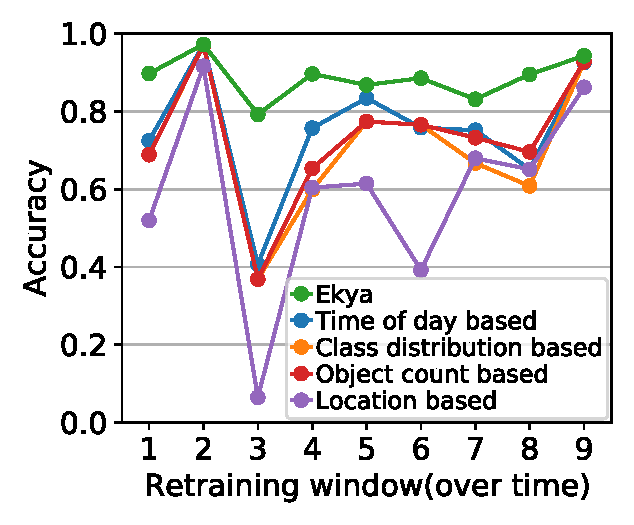
\includegraphics[width=\linewidth]{ekya/results/reuse_cached_model/new_sf_060_069_golden_label.pdf}
    \caption{\small \revtext{\name vs. re-using cached models over time}}
    \label{fig:reuse-cached-model-1}
  \end{subfigure}
  ~
  \begin{subfigure}[t]{0.48\linewidth}
    \centering
    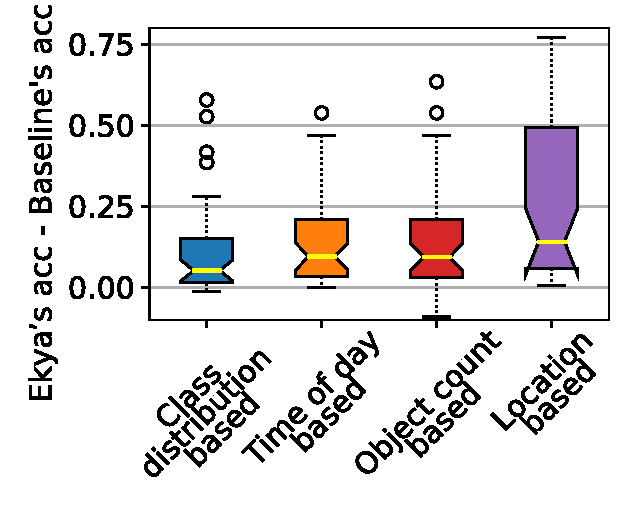
\includegraphics[width=\linewidth]{ekya/results/reuse_cached_model/new_waymo_reuse_cached_model_boxplot.pdf} 
    \caption{\small \cameratext{Average gains in accuracy across video streams} 
    %\ga{Can we change y-axis to just be direct? (Ekya's accuracy - Baseline's accuracy)}
    }
    \label{fig:reuse-cached-model-2}
  \end{subfigure}
%   \caption{\small \bf \revtext{Re-using cached models vs using \name. (a) plots the accuracy over different retraining windows as time progresses. Models retrained with \name are robust to data-drift and are able to maintain a consistently high accuracy, compared to cached-model selection techniques.}
    \caption{\small \bf \revtext{\name vs. re-using cached models. Compared to cached-model selection techniques, models retrained with \name maintain a consistently high accuracy, since it fully leverages the latest training data and is thus more robust to data-drift.}
  % \romil{1) Pick a graph which has more diversity in the baseline results 2) Why are we better? Is there some data/more plots we can use to show why the baselines are worse/ekya is better? (e.g. Training with same class distribution does not give good accuracy. Why - because the data is different)}
  }
  \label{fig:reuse-cached-model}
\end{figure}


% \junchen{mention the baseline of sending all images to the server}

\mypara{Ekya vs. Re-using pretrained models}
\revtext{An alternative to continuous retraining is to cache {\em pretrained} models and reuse them. We pre-train and cache a few tens of DNNs from earlier windows of the Waymo dataset and test four heuristics for selecting cached models. 
% - class-distribution based, time-of-day based, location based and object-count based. 
{\em Class-distribution}-based selection picks the cached DNN whose training data class distribution has the closest Euclidean distance with the current window's data. 
{\em Time-of-day}-based selection picks the cached DNN whose training data time matches the current window.
{\em Object-count}-based selection picks the cached DNN based on similar count of objects. % whose object count of its training data is closest to the current window. 
{\em Location}-based selection picks the cached DNNs trained on the same city as the current window.

Figure~\ref{fig:reuse-cached-model-1} highlights the advantages of \name over different model selection schemes. 
We find that since time-of-day-based, object-count-based, and location-based model selection techniques are agnostic to the class distributions of training data of cached models, the selected cached models sometimes do not cover all classes in the current window. 
% Since time-of-day-based, object-count-based, and location-based model selection techniques have no constraint on class distribution of training data of cached models, these heuristics often select models trained on past data which do not cover all classes in the current testing data. 
Even if we take class distribution into account when picking cached models, there are still substantial discrepancies in the appearances of objects between the current window and the history training data. %testing data and the history training data that match on all four heuristics with the current testing data.
% The class-distribution-based model selection picks models based on the class distribution similarity and thus has better average test accuracy, but it cannot guarantee the similarity of object appearance across windows. 
For instance, object appearance can vary due to pose variations, occlusion or different lighting conditions. \cameratext{In Window 3 (Figure~\ref{fig:reuse-cached-model-1}), not only are certain classes underrepresented in the training data, but the lighting conditions are also adverse.}
% \ga{Can we say that a combination of the above heuristics also do not work as well as Ekya?} 
% Moreover, the choice of similarity metric strongly affects the effect of model selection. For instance, measuring the euclidean distance between two class distribution vectors account only for absolute differences and fails to differentiate positive or negative changes. But the model selected based on this similarity metric may have distinct testing accuracy. 
\cameratext{Figure~\ref{fig:reuse-cached-model-2} presents a box plot of the accuracy difference between \name and model selection schemes, where the edges of the box represent the first and third quartiles, the waist is the median, the whiskers represent the maximum and minimum values and the circles represent any outliers.} \name's continuous retraining of models is robust to scene specific data-drifts and achieves upto 26\% higher mean accuracy.}

% \zhengxu{Since time-of-day-based, object-count-based, and location-based model selection techniques have no constraint on class distribution of training data of cached models, these heuristics often select models trained on past data which fail to cover all classes in the current testing data. Then the cached model selected leads to a low test accuracy in current window. Although the class-distribution-based model selection technique has requirements on the class distribution similarity and has better average test accuracy than other model selection techniques, it cannot guarantee the similarity of object appearance between the window used to train a cached model and the current testing window. For example, different angle, different degree of object occlusion, different lightning condition due to different time of day and different weather can harm the inference accuracy of the cached models. Additionally, the choice of similarity metric strongly affects the effect of model selection. For instance, the current choice of euclidean distance between two class distribution vector fails to differentiate 10\% more or 10\% less change in a class. But the model selected based on this similarity metric may have distinct testing accuracy.} 
%This is because even though the class distributions may be similar, the models cannot be directly reused from any window as the appearances of objects may still differ considerably (Figure \ref{fig:cityscapes-motivation}).}








